% Connectome-wired world models, v2 (reorganised around: prior work, why this distillation,
% single vs multiple connectomes, sparse vs dense, benchmarks, baselines, novelty).
\documentclass[10pt,twocolumn,letterpaper]{article}
\usepackage[review]{cvpr}   % CVPR review template (line numbers, paper-ID header); use [pagenumbers] for arXiv
\usepackage{caption}
\usepackage{booktabs}
\usepackage{multirow}
\usepackage{amsmath,amssymb}
\usepackage{graphicx}
\usepackage{xspace}
\usepackage{microtype}
\usepackage{tikz}
\usetikzlibrary{arrows.meta,positioning,shapes.geometric,calc,fit,backgrounds,decorations.pathmorphing}
\usepackage{xcolor}
\usepackage{array}

\newcommand{\todo}[1]{{\color{red}#1}}
\newcommand{\TODO}[1]{\textbf{\color{red}[TODO: #1]}}
\newcommand{\method}{CxWM\xspace}
\newcommand{\vjepa}{V-JEPA~2.1\xspace}
\newcommand{\flywire}{FlyWire\xspace}
\providecommand{\etal}{\emph{et al}.\xspace}
\providecommand{\ie}{\emph{i.e}.\xspace}
\providecommand{\eg}{\emph{e.g}.\xspace}
\newcommand{\degree}{$^\circ$}
\let\mathpm\pm
\renewcommand{\pm}{\ensuremath{\mathpm}}
\setlength{\abovecaptionskip}{.5em}
\renewcommand{\paragraph}[1]{\vspace{.4em}\noindent\textbf{#1.}}

% diagram colours (populations match the released 3-D viewer)
\definecolor{cVIS}{RGB}{66,133,244}
\definecolor{cCX}{RGB}{244,160,0}
\definecolor{cMB}{RGB}{52,168,83}
\definecolor{cOUT}{RGB}{219,68,155}
\definecolor{cTeach}{RGB}{90,90,90}
\tikzset{
  box/.style={draw,rounded corners=2pt,minimum height=1.6em,inner sep=4pt,font=\small,align=center},
  pop/.style={box,fill=#1!15,draw=#1!80!black,thick},
  arr/.style={-{Latex[length=2mm]},thick},
  darr/.style={-{Latex[length=2mm]},thick,dashed},
  lbl/.style={font=\scriptsize,align=center},
}

% generated by scripts/make_paper_tables.py; do not edit
\newcommand{\nGruArenaMse}{0.435}
\newcommand{\nGruArenaCos}{0.72}
\newcommand{\nGruTnMse}{0.430}
\newcommand{\nGruTnCos}{0.71}
\newcommand{\nGruNycMse}{0.588}
\newcommand{\nGruNycCos}{0.53}
\newcommand{\nTfArenaMse}{0.502}
\newcommand{\nTfArenaCos}{0.67}
\newcommand{\nTfTnMse}{0.502}
\newcommand{\nTfTnCos}{0.66}
\newcommand{\nTfNycMse}{0.605}
\newcommand{\nTfNycCos}{0.51}
\newcommand{\nGruRecArenaMse}{0.501}
\newcommand{\nGruRecArenaCos}{0.67}
\newcommand{\nDenseArenaMse}{0.562}
\newcommand{\nDenseArenaCos}{0.63}
\newcommand{\nNosignArenaMse}{0.573}
\newcommand{\nNosignArenaCos}{0.63}
\newcommand{\nRandsignArenaMse}{0.578}
\newcommand{\nRandsignArenaCos}{0.62}
\newcommand{\nConnArenaMse}{0.579}
\newcommand{\nConnArenaCos}{0.62}
\newcommand{\nConnTnMse}{0.571}
\newcommand{\nConnTnCos}{0.61}
\newcommand{\nConnNycMse}{0.636}
\newcommand{\nConnNycCos}{0.47}
\newcommand{\nHybridArenaMse}{0.579}
\newcommand{\nHybridArenaCos}{0.62}
\newcommand{\nRandomArenaMse}{0.583}
\newcommand{\nRandomArenaCos}{0.61}
\newcommand{\nRandomTnMse}{0.582}
\newcommand{\nRandomTnCos}{0.60}
\newcommand{\nRandomNycMse}{0.639}
\newcommand{\nRandomNycCos}{0.47}
\newcommand{\nBlockArenaMse}{0.585}
\newcommand{\nBlockArenaCos}{0.61}
\newcommand{\nBlockTnMse}{0.578}
\newcommand{\nBlockTnCos}{0.60}
\newcommand{\nBlockNycMse}{0.665}
\newcommand{\nBlockNycCos}{0.44}
\newcommand{\nDegreeArenaMse}{0.610}
\newcommand{\nDegreeArenaCos}{0.59}
\newcommand{\nDegreeNycMse}{0.731}
\newcommand{\nDegreeNycCos}{0.45}
\newcommand{\nConnAttnArenaMse}{0.727}
\newcommand{\nConnAttnArenaCos}{0.48}
\newcommand{\nBlockAttnArenaMse}{0.733}
\newcommand{\nBlockAttnArenaCos}{0.47}
\newcommand{\nGruAttnArenaMse}{0.448}
\newcommand{\nGruAttnArenaCos}{0.71}
\newcommand{\nTfAttnArenaMse}{0.504}
\newcommand{\nTfAttnArenaCos}{0.67}
\newcommand{\nCopyLastArenaMse}{0.811}
\newcommand{\nCopyLastTnMse}{0.806}
\newcommand{\nCopyLastNycMse}{0.607}
\newcommand{\nConstMeanArenaMse}{0.992}
\newcommand{\nConstMeanTnMse}{0.968}
\newcommand{\nConstMeanNycMse}{0.843}
\newcommand{\nGruArenaHd}{30.3}
\newcommand{\nGruArenaPos}{0.41}
\newcommand{\nGruTnHd}{33.7}
\newcommand{\nGruTnPos}{0.36}
\newcommand{\nGruNycHd}{29.9}
\newcommand{\nGruNycPos}{0.37}
\newcommand{\nTfArenaHd}{34.3}
\newcommand{\nTfArenaPos}{0.40}
\newcommand{\nTfTnHd}{37.2}
\newcommand{\nTfTnPos}{0.39}
\newcommand{\nTfNycHd}{30.6}
\newcommand{\nTfNycPos}{0.38}
\newcommand{\nGruRecArenaHd}{35.5}
\newcommand{\nGruRecArenaPos}{0.30}
\newcommand{\nDenseArenaHd}{21.3}
\newcommand{\nDenseArenaPos}{0.68}
\newcommand{\nNosignArenaHd}{13.8}
\newcommand{\nNosignArenaPos}{0.88}
\newcommand{\nRandsignArenaHd}{9.2}
\newcommand{\nRandsignArenaPos}{0.94}
\newcommand{\nConnArenaHd}{9.4}
\newcommand{\nConnArenaPos}{0.94}
\newcommand{\nConnTnHd}{15.1}
\newcommand{\nConnTnPos}{0.90}
\newcommand{\nConnNycHd}{10.6}
\newcommand{\nConnNycPos}{0.94}
\newcommand{\nHybridArenaHd}{8.6}
\newcommand{\nHybridArenaPos}{0.94}
\newcommand{\nRandomArenaHd}{12.8}
\newcommand{\nRandomArenaPos}{0.88}
\newcommand{\nRandomTnHd}{17.8}
\newcommand{\nRandomTnPos}{0.83}
\newcommand{\nRandomNycHd}{12.1}
\newcommand{\nRandomNycPos}{0.88}
\newcommand{\nBlockArenaHd}{10.9}
\newcommand{\nBlockArenaPos}{0.93}
\newcommand{\nBlockTnHd}{16.4}
\newcommand{\nBlockTnPos}{0.89}
\newcommand{\nBlockNycHd}{11.9}
\newcommand{\nBlockNycPos}{0.91}
\newcommand{\nDegreeArenaHd}{12.7}
\newcommand{\nDegreeArenaPos}{0.89}
\newcommand{\nDegreeNycHd}{14.3}
\newcommand{\nDegreeNycPos}{0.84}
\newcommand{\nConnAttnArenaHd}{9.8}
\newcommand{\nConnAttnArenaPos}{0.93}
\newcommand{\nBlockAttnArenaHd}{13.5}
\newcommand{\nBlockAttnArenaPos}{0.89}
\newcommand{\nGruAttnArenaHd}{31.4}
\newcommand{\nGruAttnArenaPos}{0.40}
\newcommand{\nTfAttnArenaHd}{34.1}
\newcommand{\nTfAttnArenaPos}{0.42}
\newcommand{\nActOnlyArenaHd}{40.1}
\newcommand{\nActOnlyTnHd}{39.7}
\newcommand{\nActOnlyNycHd}{15.7}
\newcommand{\nIntegratorArenaHd}{0.0}
\newcommand{\nIntegratorTnHd}{11.1}
\newcommand{\nIntegratorNycHd}{0.0}
\newcommand{\nGruArenaMlpHd}{27.2}
\newcommand{\nGruArenaDarkSixteenHd}{38.8}
\newcommand{\nGruArenaDarkTwentyHd}{27.9}
\newcommand{\nTfArenaMlpHd}{30.4}
\newcommand{\nTfArenaDarkSixteenHd}{44.6}
\newcommand{\nGruRecArenaMlpHd}{32.4}
\newcommand{\nGruRecArenaDarkSixteenHd}{44.8}
\newcommand{\nGruRecArenaDarkTwentyHd}{33.7}
\newcommand{\nDenseArenaMlpHd}{41.2}
\newcommand{\nDenseArenaDarkSixteenHd}{29.9}
\newcommand{\nDenseArenaDarkTwentyHd}{21.3}
\newcommand{\nRandsignArenaMlpHd}{4.7}
\newcommand{\nRandsignArenaDarkSixteenHd}{18.6}
\newcommand{\nRandsignArenaDarkTwentyHd}{13.6}
\newcommand{\nConnArenaMlpHd}{5.4}
\newcommand{\nConnArenaDarkSixteenHd}{18.5}
\newcommand{\nConnArenaDarkTwentyHd}{12.6}
\newcommand{\nHybridArenaMlpHd}{5.2}
\newcommand{\nHybridArenaDarkSixteenHd}{17.6}
\newcommand{\nRandomArenaMlpHd}{7.1}
\newcommand{\nRandomArenaDarkSixteenHd}{25.4}
\newcommand{\nRandomArenaDarkTwentyHd}{17.3}
\newcommand{\nBlockArenaMlpHd}{5.6}
\newcommand{\nBlockArenaDarkSixteenHd}{23.7}
\newcommand{\nBlockArenaDarkTwentyHd}{15.9}
\newcommand{\nDegreeArenaMlpHd}{6.9}
\newcommand{\nDegreeArenaDarkSixteenHd}{24.0}
\newcommand{\nDegreeArenaDarkTwentyHd}{17.2}
\newcommand{\nConnAttnArenaMlpHd}{7.2}
\newcommand{\nConnAttnArenaDarkSixteenHd}{20.1}
\newcommand{\nBlockAttnArenaMlpHd}{7.8}
\newcommand{\nBlockAttnArenaDarkSixteenHd}{26.9}
\newcommand{\nGruAttnArenaMlpHd}{28.7}
\newcommand{\nGruAttnArenaDarkSixteenHd}{40.3}
\newcommand{\nTfAttnArenaMlpHd}{30.5}
\newcommand{\nTfAttnArenaDarkSixteenHd}{43.4}
\newcommand{\nGruArenaCloser}{18}
\newcommand{\nGruArenaSucc}{0.13}
\newcommand{\nGruTnCloser}{19}
\newcommand{\nGruTnSucc}{0.11}
\newcommand{\nGruNycCloser}{19}
\newcommand{\nGruNycSucc}{0.12}
\newcommand{\nTfArenaCloser}{12}
\newcommand{\nTfArenaSucc}{0.10}
\newcommand{\nTfTnCloser}{17}
\newcommand{\nTfTnSucc}{0.05}
\newcommand{\nGruRecArenaCloser}{29}
\newcommand{\nGruRecArenaSucc}{0.15}
\newcommand{\nDenseArenaCloser}{36}
\newcommand{\nDenseArenaSucc}{0.11}
\newcommand{\nNosignArenaCloser}{47}
\newcommand{\nNosignArenaSucc}{0.13}
\newcommand{\nConnArenaCloser}{43}
\newcommand{\nConnArenaSucc}{0.11}
\newcommand{\nConnTnCloser}{37}
\newcommand{\nConnTnSucc}{0.13}
\newcommand{\nConnNycCloser}{50}
\newcommand{\nConnNycSucc}{0.47}
\newcommand{\nHybridArenaCloser}{49}
\newcommand{\nHybridArenaSucc}{0.15}
\newcommand{\nRandomArenaCloser}{41}
\newcommand{\nRandomArenaSucc}{0.16}
\newcommand{\nRandomTnCloser}{34}
\newcommand{\nRandomTnSucc}{0.10}
\newcommand{\nBlockArenaCloser}{40}
\newcommand{\nBlockArenaSucc}{0.13}
\newcommand{\nBlockTnCloser}{41}
\newcommand{\nBlockTnSucc}{0.17}
\newcommand{\nBlockNycCloser}{54}
\newcommand{\nBlockNycSucc}{0.51}
\newcommand{\nDegreeArenaCloser}{42}
\newcommand{\nDegreeArenaSucc}{0.14}
\newcommand{\nConnAttnArenaCloser}{40}
\newcommand{\nConnAttnArenaSucc}{0.10}
\newcommand{\nBlockAttnArenaCloser}{37}
\newcommand{\nBlockAttnArenaSucc}{0.15}
\newcommand{\nGruAttnArenaCloser}{22}
\newcommand{\nGruAttnArenaSucc}{0.07}
\newcommand{\nTfAttnArenaCloser}{24}
\newcommand{\nTfAttnArenaSucc}{0.11}
\newcommand{\nGruArenaRvMse}{9.94}
\newcommand{\nGruArenaRvFtMse}{1.18}
\newcommand{\nGruArenaRvTransferHd}{84.1}
\newcommand{\nGruArenaRvIndomainHd}{7.6}
\newcommand{\nGruNycRvMse}{5.57}
\newcommand{\nDenseArenaRvMse}{9.73}
\newcommand{\nDenseArenaRvFtMse}{1.21}
\newcommand{\nDenseArenaRvTransferHd}{29.5}
\newcommand{\nDenseArenaRvIndomainHd}{9.1}
\newcommand{\nNosignArenaRvMse}{9.59}
\newcommand{\nNosignArenaRvFtMse}{1.26}
\newcommand{\nNosignArenaRvTransferHd}{24.3}
\newcommand{\nNosignArenaRvIndomainHd}{7.7}
\newcommand{\nConnArenaRvMse}{9.68}
\newcommand{\nConnArenaRvFtMse}{1.24}
\newcommand{\nConnArenaRvTransferHd}{30.9}
\newcommand{\nConnArenaRvIndomainHd}{7.7}
\newcommand{\nConnNycRvMse}{6.10}
\newcommand{\nRandomArenaRvMse}{9.56}
\newcommand{\nRandomArenaRvFtMse}{1.26}
\newcommand{\nRandomArenaRvTransferHd}{79.1}
\newcommand{\nRandomArenaRvIndomainHd}{9.9}
\newcommand{\nRandomNycRvMse}{6.00}
\newcommand{\nDegreeArenaRvMse}{9.69}
\newcommand{\nDegreeArenaRvFtMse}{1.25}
\newcommand{\nDegreeArenaRvTransferHd}{88.7}
\newcommand{\nDegreeArenaRvIndomainHd}{7.1}
\newcommand{\nDegreeNycRvMse}{6.01}
\newcommand{\nCopyLastRvMse}{0.84}
\newcommand{\nConstMeanRvMse}{10.28}
\newcommand{\nActOnlyRvHd}{4.7}
\newcommand{\nGruBetterArena}{25}
\newcommand{\nTfBetterArena}{13}
\newcommand{\nConnOverBlockArena}{1.0}
\newcommand{\nConnBlockGapArena}{1.5}
\newcommand{\nConnBlockGapArenaDarkSixteen}{5.2}
\newcommand{\nGruBetterTn}{25}
\newcommand{\nTfBetterTn}{12}
\newcommand{\nConnOverBlockTn}{1.2}
\newcommand{\nConnBlockGapTn}{1.3}
\newcommand{\nConnBlockGapTnDarkSixteen}{4.3}
\newcommand{\nGruBetterNyc}{8}
\newcommand{\nTfBetterNyc}{5}
\newcommand{\nConnOverBlockNyc}{4.4}
\newcommand{\nConnBlockGapNyc}{1.3}
\newcommand{\nConnBlockGapNycDarkSixteen}{4.9}
\newcommand{\nSeeds}{5}
\newcommand{\nSeedsNyc}{3}
\newcommand{\nSeedsTn}{3}
\newcommand{\nRvClips}{8}
\newcommand{\nRvEpisodes}{79}
\newcommand{\nCheckpoints}{17}
          % numbers generated from results/ by scripts/make_paper_tables.py
% placeholders for numbers run 2 has not produced yet (real-video stage and transformer NYC homing; box stopped 2026-11-05 18:00)
\providecommand{\nConnRvFtMse}{\TODO{ConnRvFtMse}}
\providecommand{\nConnRvIndomainHd}{\TODO{ConnRvIndomainHd}}
\providecommand{\nConnRvMse}{\TODO{ConnRvMse}}
\providecommand{\nConnRvTransferHd}{\TODO{ConnRvTransferHd}}
\providecommand{\nGruRvFtMse}{\TODO{GruRvFtMse}}
\providecommand{\nGruRvIndomainHd}{\TODO{GruRvIndomainHd}}
\providecommand{\nGruRvMse}{\TODO{GruRvMse}}
\providecommand{\nGruRvTransferHd}{\TODO{GruRvTransferHd}}
\providecommand{\nTfNycSucc}{\TODO{TfNycSucc}}
  % \TODO placeholders for numbers run 2 has not produced yet
\definecolor{cvprblue}{rgb}{0.21,0.49,0.74}
\usepackage[breaklinks,colorlinks,allcolors=cvprblue]{hyperref}
\def\confName{CVPR}
\def\confYear{2027}

\title{Distilling a Video World Model into the \emph{Drosophila} Connectome:\\
What a Real Wiring Diagram Buys a Latent Predictor}

\author{Anonymous CVPR submission\\
Paper ID *****
}

\begin{document}
\maketitle
\begin{abstract}
A fruit fly keeps its heading and a vector home for seconds in darkness with a few thousand neurons whose wiring is
now known synapse by synapse. We ask whether that wiring is a useful prior for a modern video world model, and we
answer with matched controls rather than a single headline number. We distil the latent dynamics of \vjepa (ViT-B),
a self-supervised video foundation model, into a leaky recurrent student whose \emph{only} recurrent connections are
the 91,663 signed synapses among 6,935 neurons of the \flywire \emph{Drosophila} connectome (visual projection, central
complex, mushroom-body output and descending populations). The student is trained on one objective, next-latent
prediction under random blackouts of the visual input, and nothing about heading, position or action is supervised.
Against six wiring controls that fix neuron count, edge count, region block structure and Dale's-law signs, against a
dense recurrence, and against a parameter-matched GRU and a parameter-matched causal transformer, the connectome is
\emph{not} the best predictor: the GRU is \nGruBetterArena\,\% better. What the wiring buys is a path-integrating
state. During 8 blind steps a ridge probe reads heading from the connectome state to \nConnArenaHd\degree\ median error
and position to $R^2$\,\nConnArenaPos, against \nGruArenaHd\degree\ and \nGruArenaPos\ for the GRU; the code survives
16 and 20 dark steps, transfers to a raycast twin of Midtown Manhattan and persists under continuous turn angles. Sparse
random and block-shuffled wirings of the same size form the code too, \nConnBlockGapArena\ to
\nConnBlockGapArenaDarkSixteen\degree\ worse, so the effect belongs to connectome-scale sparse signed recurrence, with a
small, reproducible bonus for the real synapse list. Coupling two or three copies of the brain through the 40,194 real
commissural synapses adds neurons but no accuracy. We release both environments, the real-video ingest pipeline, the
training and evaluation code and all checkpoints.
\end{abstract}

\section{Introduction}
\label{sec:intro}

\begin{figure*}[t]
  \centering
  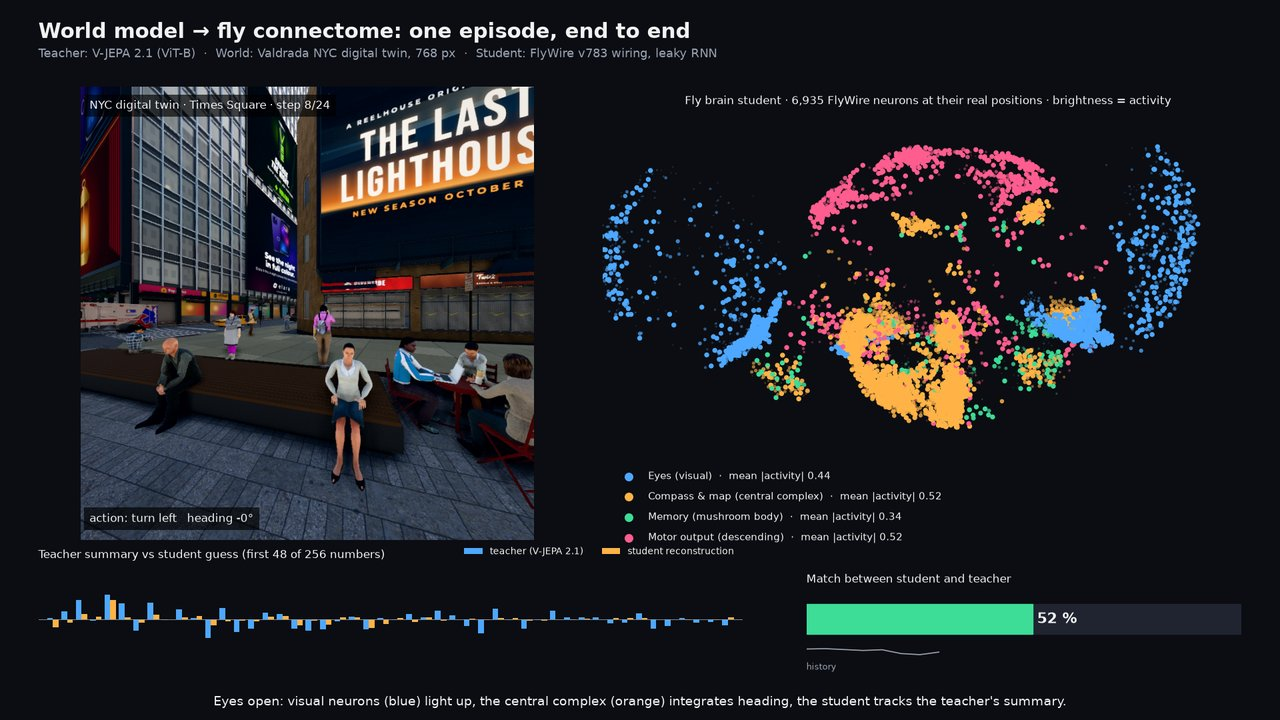
\includegraphics[width=0.495\linewidth]{fig/e2e_t07.jpg}\hfill
  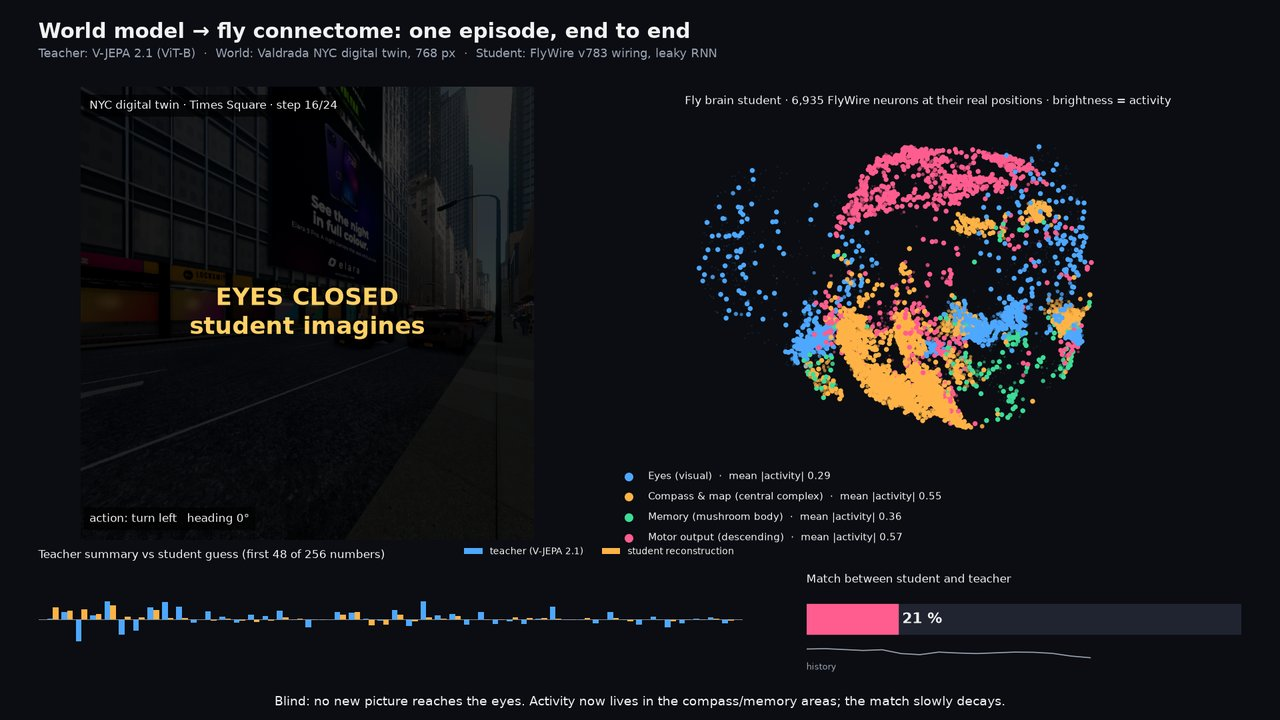
\includegraphics[width=0.495\linewidth]{fig/e2e_t15.jpg}
  \caption{\textbf{One episode, end to end, in the Manhattan twin.} Left: eyes open at step 8; the view the teacher
  encodes, the connectome student's activity drawn on the real \flywire soma positions (blue VIS, orange CX, green MB,
  pink OUT), the teacher's latent next to the student's reconstruction, and the match gauge. Right: eyes closed at step
  16; no new picture reaches the eyes, activity moves into the compass and memory populations, and the match decays
  slowly while the state keeps heading and position (\cref{sec:probes}). Full video in the supplement.}
  \label{fig:teaser}
\end{figure*}

\begin{figure*}[t]
  \centering
  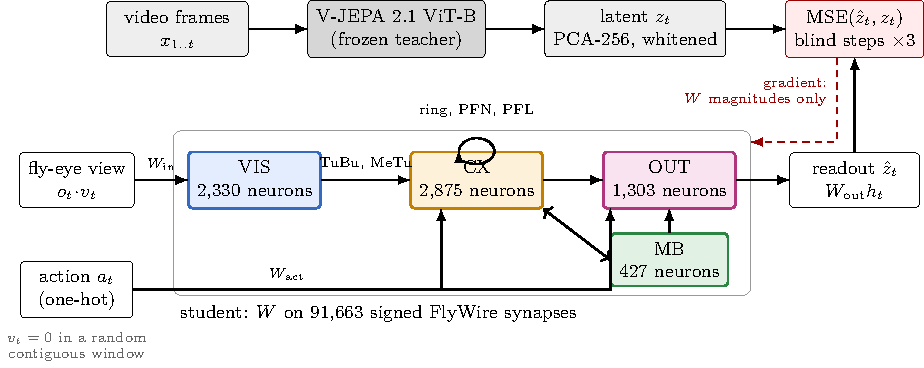
\includegraphics[width=\linewidth]{fig/pipeline.pdf}  % source: fig/src/pipeline.tex (build: fig/src/build.sh)
  \caption{\textbf{Pipeline.} A frozen \vjepa encoder turns each frame into a causal latent $z_t$. The student is a leaky
  rate network whose recurrence lives only on the signed synapses of four \flywire populations; training can rescale a
  synapse but never flip its sign, add one or remove one. The only training signal is next-latent prediction, with the
  view cut in a random window so the state must carry the latent on the action record alone. Heading, position and
  homing are read out of the trained state afterwards and were never supervised.}
  \label{fig:pipeline}
\end{figure*}

Ask a world model to imagine the next second of a video and it will do a reasonable job. Ask it what it imagines after
the lights go out, and the answer depends on what its recurrent core chose to remember. In most video world models that
core is a generic block, a GRU or a transformer layer, sized by compute and shaped only by the prediction
loss~\cite{ha2018world,hafner2023dreamerv3,assran2025vjepa2}. Biology solved the same problem differently. A fruit fly in
darkness holds its heading and a vector back to its start for many seconds using a few thousand central-complex
neurons, and the complete synapse-level wiring of that circuit is now
public~\cite{seelig2015neural,green2017neural,turnerevans2017angular,dorkenwald2024neuronal,schlegel2024whole}.

This paper puts the two together and asks one plain question: \emph{if a world model's recurrence is forced to be the
fly's wiring diagram, what does the wiring buy?} We distil \vjepa~\cite{assran2025vjepa2} into a leaky rate network of
6,935 \flywire neurons whose only recurrent weights sit on the 91,663 signed synapses of the real connectome
(\cref{fig:pipeline}). The student never sees the teacher's weights, only its latent through the loss, and is trained on
one objective: next-latent prediction under random blackouts of the visual input.

\paragraph{Why distillation, and why this kind}
Three alternatives were available and rejected. Training the connectome network directly on pixels would entangle the
wiring question with representation learning; fitting it to neural recordings, as prior connectome models
do~\cite{lappalainen2024connectome}, would answer a neuroscience question rather than a world-model question; and
distilling into a free architecture, as world-model compression does~\cite{hinton2015distilling,kasai2021t2r}, would
leave the wiring unconstrained. Latent-regression distillation from a frozen video encoder (the recipe of
DINO-WM~\cite{zhou2024dinowm} and JEPA world models~\cite{assran2025vjepa2}) is the one setting in which the student's
recurrence can be fixed to a biological graph while the target stays a strong, general, self-supervised representation.

\paragraph{What we find}
The answer has two halves, and we state both plainly. The wiring is \emph{not} a better predictor: against controls that
hold neuron count, edge count, region block structure, Dale's-law signs and parameter count fixed, the real connectome
beats its shuffled twins by about one percent of latent error, consistently, while a parameter-matched GRU is
\nGruBetterArena\,\% better. What the wiring buys is a \emph{path-integrating state} (\cref{fig:main}): during the blind
steps a ridge probe reads heading from the connectome state to \nConnArenaHd\degree\ median error and position to
$R^2$\,\nConnArenaPos, where the better-predicting GRU gives \nGruArenaHd\degree\ and \nGruArenaPos. The code survives 16
and 20 dark steps, reappears in a raycast twin of Manhattan, widens under a non-linear probe and persists under
continuous turn angles. Sparse random and block-shuffled wirings form it too, \nConnBlockGapArena\ to
\nConnBlockGapArenaDarkSixteen\degree\ worse: the exact synapse list is a small reproducible bonus, not the cause.

\begin{figure*}[t]
  \centering
  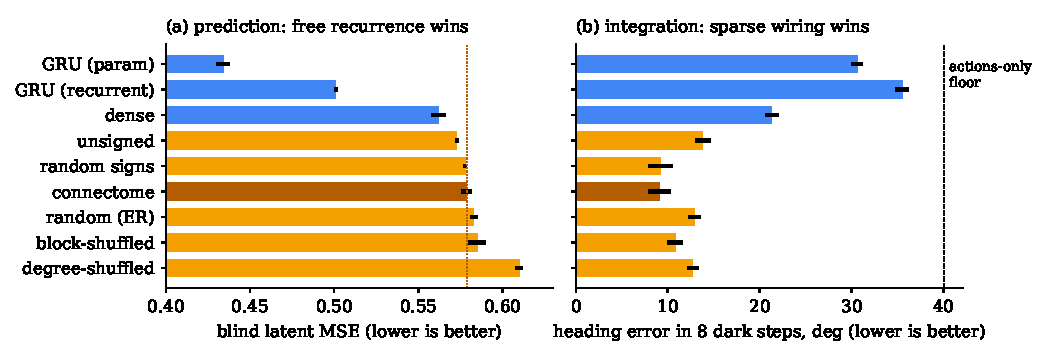
\includegraphics[width=\linewidth]{fig/ladder.pdf}
  \caption{\textbf{The wiring makes a worse predictor and a better integrator} (arena, mean\pm sd over 5 seeds).
  (a) Blind latent-prediction error: every free recurrence (blue) beats every fixed sparse graph (orange); the real
  connectome (dark) beats its shuffled twins by about one percent. (b) Median heading error decoded from the state
  during 8 dark steps: the ordering flips. Sparse signed graphs hold heading to about 10\degree, the GRUs to over
  30\degree, against a 40\degree\ floor for a linear readout of the actions alone.}
  \label{fig:main}
\end{figure*}

\paragraph{Contributions}
\begin{itemize}
  \item A distillation recipe that turns a video foundation model into a world model whose recurrence is a fixed,
        signed, biologically sourced sparse graph, with controls that separate wiring identity from density, degree
        sequence, region structure and sign structure (\cref{sec:method}).
  \item A single-versus-multiple-connectome study: $K$ copies of the brain coupled only through the 40,194 real
        commissural synapses, showing that neuron count is not the limiting resource (\cref{sec:multi}).
  \item The first demonstration, to our knowledge, that a connectome-wired latent predictor forms a linearly readable
        heading and position code in the dark that neither a GRU nor a transformer trained on the same objective forms,
        with information-ceiling, continuous-turn, feature-count and non-linearity controls (\cref{sec:probes}).
  \item A behavioural test of that code (blind homing, goal-vector navigation) with oracle, dead-reckoning and random
        controls, reported in full including the negative outcomes, plus real phone video as a third world
        (\cref{sec:behaviour,sec:realvid}).
  \item Two simulated environments, the real-video ingest pipeline, all code and checkpoints, released.
\end{itemize}

\section{Prior work and where this paper sits}
\label{sec:related}

\begin{table*}[t]
  \centering\small
  \caption{\textbf{Prior work along the three axes this paper joins.} Each row asks: is the teacher a self-supervised
  video model, is the student's recurrence fixed by biology, and is the student evaluated as a world model (blind
  prediction, planning or homing)? Only the last row has all three.}
  \label{tab:prior}
  \begin{tabular}{p{4.2cm}p{4.6cm}ccc}
    \toprule
    work & what it does & video-FM teacher & bio.\ recurrence & WM eval \\
    \midrule
    DreamerV3~\cite{hafner2023dreamerv3,hafner2025dreamerv3nature}, IRIS~\cite{micheli2023iris}, STORM~\cite{zhang2023storm} & learn a latent dynamics model with a free GRU / transformer core & -- & -- & \checkmark \\
    V-JEPA 2 / 2.1~\cite{assran2025vjepa2,vjepa21_2026}, DINO-WM~\cite{zhou2024dinowm}, NWM~\cite{bar2024nwm} & frozen self-supervised encoder plus a learned predictor; plan in latent space & \checkmark & -- & \checkmark \\
    KD, FitNets, DINOv2 / TinyViT distillation~\cite{hinton2015distilling,romero2015fitnets,oquab2024dinov2,wu2022tinyvit} & compress a model into a smaller member of the same family & (\checkmark) & -- & -- \\
    Transformer$\to$RNN / SSM distillation~\cite{kasai2021t2r,katharopoulos2020linear,bick2024transformers,wang2024mamballama} & change the architecture family of the student; recurrence stays free & -- & -- & -- \\
    Policy distillation / imagination~\cite{rusu2016policy,hafner2020dreamer} & distil behaviour, not dynamics & -- & -- & (\checkmark) \\
    Connectome-constrained vision~\cite{lappalainen2024connectome}, whole-brain LIF~\cite{shiu2024drosophila} & fit the wiring to neural recordings or a hand-designed task & -- & \checkmark & -- \\
    Neural circuit policies~\cite{lechner2020neural}, bio-instantiated RNNs~\cite{goulas2021bio} & small RNNs with wiring borrowed from C.~elegans or cortical atlases & -- & \checkmark & -- \\
    Path-integration RNNs~\cite{cueva2018emergence,banino2018vector,sorscher2019unified} & heading / grid codes emerge when the task is localisation & -- & -- & -- \\
    \midrule
    \textbf{this paper} & distil \vjepa into the \flywire wiring; matched controls; probes and blind homing & \checkmark & \checkmark & \checkmark \\
    \bottomrule
  \end{tabular}
\end{table*}

\paragraph{Vision world models}
Following the taxonomy of Yu \etal~\cite{yu2026seeing}, vision world models fall into sequential token
generation~\cite{bruce2024genie}, diffusion generation~\cite{agarwal2025cosmos,bar2024nwm}, embedding
prediction~\cite{lecun2022path,bardes2024vjepa,assran2025vjepa2,vjepa21_2026,zhou2024dinowm,baldassarre2025dinoworld}
and latent state transition~\cite{ha2018world,hafner2023dreamerv3,micheli2023iris,zhang2023storm,robine2023twm}. Our
student is an embedding-prediction model with a state-transition core: a frozen \vjepa encoder supplies the target
space, as DINO-WM does with frozen DINO features, and a recurrent network carries the latent through time under
actions, as Dreamer's recurrent state-space model does. In every one of these systems the recurrent core is a free
architectural choice sized by compute. Ours is fixed by a wiring diagram, so we compare against the two cores a reader
would ask for by name, a GRU~\cite{cho2014learning} and a causal transformer predictor, both matched to the student's
parameter budget, and against the trivial copy-last and constant predictors every world-model benchmark
reports~\cite{bar2024nwm}.

\paragraph{Distillation}
Knowledge distillation~\cite{hinton2015distilling,romero2015fitnets} and its vision-foundation-model
descendants~\cite{oquab2024dinov2,wu2022tinyvit} compress a model into a smaller member of the same family. A second
line changes the family, converting transformers into RNNs or state-space models by matching hidden states and
outputs~\cite{katharopoulos2020linear,kasai2021t2r,bick2024transformers,wang2024mamballama}; a third distils behaviour
rather than dynamics~\cite{rusu2016policy,hafner2020dreamer}. In all of them the student's recurrence remains free to
take whatever shape the loss prefers. Our student's recurrence cannot: its sparsity pattern, its signs and its
neuron count are fixed before training. The recipe we use, latent regression from a frozen encoder, is deliberately
the plainest member of the family so that any difference between students is attributable to wiring.

\paragraph{Connectome-constrained models}
Whole-brain \emph{Drosophila} connectomes~\cite{dorkenwald2024neuronal,schlegel2024whole} with predicted
neurotransmitter signs~\cite{eckstein2024neurotransmitter} have enabled models whose connectivity is read off the wiring
diagram. Lappalainen \etal~\cite{lappalainen2024connectome} fit a connectome-constrained visual system on a motion task
and predict recordings; Shiu \etal~\cite{shiu2024drosophila} simulate the whole brain as leaky integrate-and-fire units;
central-complex models~\cite{hulse2021connectome,stone2017anatomically} explain heading and path integration
mechanistically; neural circuit policies~\cite{lechner2020neural} and bio-instantiated RNNs~\cite{goulas2021bio} borrow
small wiring motifs for control. These fit neural data or hand-designed tasks. We instead distil a self-supervised video
model into the wiring and measure what the wiring does to a world model, with matched-control analysis as the main
instrument.

\paragraph{Path integration in artificial networks}
RNNs trained to localise from velocity develop grid- and head-direction-like
codes~\cite{cueva2018emergence,banino2018vector,sorscher2019unified}, and the fly's ring attractor is the biological
reference~\cite{seelig2015neural,kim2017ring,green2017neural,turnerevans2017angular}. In those studies the task \emph{is}
localisation. Here the task is latent video prediction; heading and position are never supervised, and whether such a
code forms turns out to depend on the recurrent topology, not only on the objective.

\paragraph{Null models and sparse recurrence}
Degree-preserving rewiring~\cite{maslov2002specificity} and Erd\H{o}s--R\'enyi graphs~\cite{erdos1959random} are the
standard nulls for network structure; we add a block-preserving variant that keeps region-to-region edge counts. The
sparse-training literature~\cite{frankle2019lottery,narang2017exploring} shows that sparse RNNs can match dense ones at
a fraction of the weights; our dense control and recurrent-budget-matched GRU place the connectome on that axis.

\section{Method}
\label{sec:method}

\subsection{Teacher: which world model and why}
The teacher is \vjepa ViT-B~\cite{assran2025vjepa2,vjepa21_2026}, a self-supervised video model trained by predicting
masked latent features rather than pixels. Three properties make it the right teacher for a wiring question. Its
latent is \emph{action-free and generic}, so nothing about navigation is baked into the target. It is \emph{causal
per step} in our use: each environment step is duplicated into a 16-frame tubelet that ends at $t$, so a blind
target never contains frames the student has not seen. And it is \emph{cheap to regress}: the mean token concatenated
with $2\times2$ pooled tokens (3,840-d) is projected to a PCA-256 basis fit on the training set (94.6\,\% variance on the
arena, 91.0\,\% on NYC) and whitened by one scalar. All MSE values are in this whitened space. The teacher's weights
are never touched; it is a target generator.

\subsection{Distillation: which technique and why}
We use response-based latent regression, the plainest member of the distillation
family~\cite{hinton2015distilling}: the student's linear readout must match the teacher's latent at every step,
\begin{equation}
  \mathcal{L} = \sum_t w_t\,\big\lVert W_{\rm out} h_t - z_t\big\rVert^2 + 10^{-4}\,\overline{h^2},
  \label{eq:loss}
\end{equation}
with $w_t=3$ on blind steps and $1$ otherwise,
and no feature-alignment, no logit or attention matching and no policy term. The blind steps are the point: during a
random contiguous window the visual input is zeroed and only the action is given, so the student must carry the
teacher's latent forward from the action record. Feature-level distillation~\cite{romero2015fitnets} was rejected
because the student has no layers to align; transformer-to-RNN hidden-state matching~\cite{bick2024transformers} was
rejected because the student's state is a set of named neurons, not a free vector. Anything the state learns about
heading or position is therefore a by-product of \cref{eq:loss}.

\subsection{Connectome subgraph}
\label{sec:connectome}
From \flywire v783~\cite{dorkenwald2024neuronal,schlegel2024whole} we take 6,935 neurons in four populations
(\cref{fig:pipeline}): VIS (2,330; TuBu, MeTu, LC and LPLC visual projection neurons), CX (2,875; every central-complex
class, including EPG, PEN, $\Delta$7, PFN, PFL, h$\Delta$, FC, ER and ExR), MB (427; mushroom-body output and
dopaminergic neurons) and OUT (1,303; descending neurons). Edges are the 91,663 directed pairs with at least 5
synapses; 40,194 of them cross the midline. Each edge's sign is the predicted neurotransmitter of its presynaptic
neuron~\cite{eckstein2024neurotransmitter} (ACh, DA, 5-HT, OA excitatory; Glu, GABA inhibitory; 49.9\,\% excitatory),
so Dale's law holds by construction. The optic lobe (about 70k neurons) is omitted because it would dominate the
neuron count while adding nothing the teacher latent does not already encode. \Cref{sec:ablation} ablates the synapse
threshold and the region choice.

\subsection{Student}
\label{sec:student}
\begin{figure}[t]
  \centering
  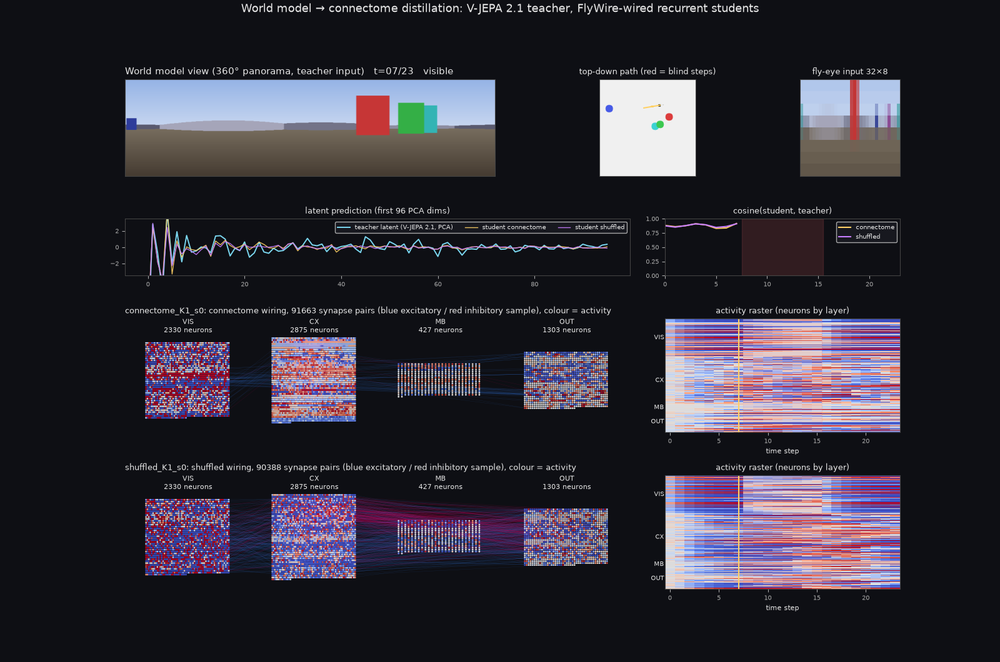
\includegraphics[width=0.49\linewidth]{fig/wm2cx_connectome_t07.png}\hfill
  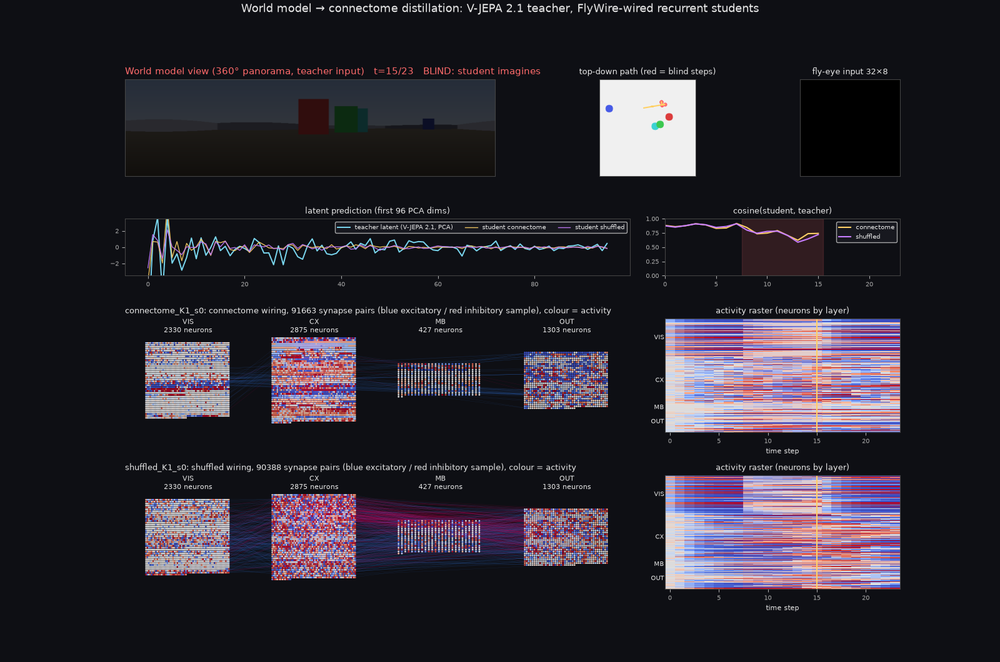
\includegraphics[width=0.49\linewidth]{fig/wm2cx_connectome_t15.png}
  \caption{\textbf{The student's state is a set of named neurons.} Activity of all 6,935 neurons at their \flywire soma
  positions, eyes open (left, step 8) and eyes closed (right, step 16) in the arena. Because every unit is a real cell
  with a cell type and a hemisphere, probes can be asked of populations (EPG, CX, VIS) and not only of the whole state.}
  \label{fig:activity}
\end{figure}
The student is a leaky tanh rate network on the connectome's neurons,
\begin{equation}
  h_{t+1} = (1-\alpha)\,h_t + \alpha\tanh\!\big(g\,(W h_t + W_{\rm in}\, o_t v_t + W_{\rm act}\, a_t + b)\big),
  \label{eq:student}
\end{equation}
with $\alpha=0.5$, gain $g$, fly-eye input $o_t$ ($32\times8\times3$) gated by the visibility flag $v_t$ and one-hot
action $a_t$. $W$ is non-zero only on connectome edges and parametrised as $W_{ij}=s_{ij}\,\mathrm{softplus}(w_{ij})$
with $s_{ij}$ fixed, so training can change synaptic strength but never sign or existence. Visual input enters VIS
neurons only; the action enters CX and OUT; the readout is linear from all neurons. The recurrence has 91,663
parameters; $W_{\rm in}$ and the readout add 3.6\,M, identical for every sparse wiring. One step costs $O(E)$.

\subsection{Single connectome versus multiple connectomes}
\label{sec:multi-method}
\begin{figure}[t]
  \centering
  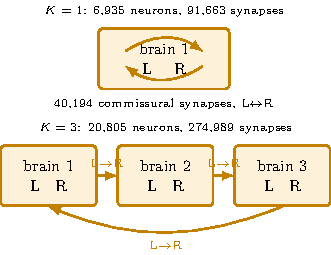
\includegraphics[width=\linewidth]{fig/multi.pdf}  % source: fig/src/multi.tex (build: fig/src/build.sh)
  \caption{\textbf{One brain or several.} For $K>1$ the whole subgraph is cloned $K$ times. Ipsilateral synapses stay
  inside each copy; each of the 40,194 contralateral synapses is moved so that it connects copy $k$ to copy $k+1$
  (modulo $K$). No new edge is invented, so the multi-brain student is still a real wiring diagram, and the input
  and readout maps are shared, so the parameter count grows only by the synapses.}
  \label{fig:multi}
\end{figure}
A single fly brain has a fixed neuron count. To ask whether the connectome is \emph{capacity}-limited rather than
\emph{wiring}-limited we clone the whole subgraph $K$ times and couple the copies through the real commissural
edges only (\cref{fig:multi}). The construction keeps every control valid: edge count scales exactly by $K$, degrees
are preserved per copy, and Dale's signs are untouched. We run $K\in\{1,2,3\}$ with five seeds each.

\subsection{Sparse state versus dense state: the controls}
\label{sec:controls}
\begin{figure}[t]
  \centering
    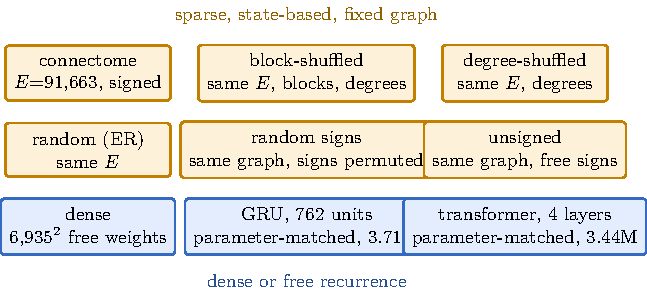
\includegraphics[width=\linewidth]{fig/controls.pdf}  % source: fig/src/controls.tex (build: fig/src/build.sh)
  \caption{\textbf{Nine recurrent cores at one input, one readout, one loss.} Orange (top two rows) cores share the neuron set,
  region labels, I/O routing, edge count and Dale-consistent sign fraction and differ only in which synapses exist or
  which neurons are excitatory. Blue (bottom row) cores are what current latent world models use. Block-shuffled is the decisive
  control: it keeps the macro-architecture and destroys only synapse identity.}
  \label{fig:controls}
\end{figure}
Every sparse control (\cref{fig:controls}) keeps the neuron set, the region labels, input and output routing, the
exact edge count, no self-loops and Dale-consistent signs at the real excitatory fraction. \textbf{Block-shuffled}
applies Maslov--Sneppen rewiring~\cite{maslov2002specificity} inside each region-to-region block, preserving per-block
in- and out-degrees and all block edge counts. \textbf{Degree-shuffled} rewires globally. \textbf{Random} is
Erd\H{o}s--R\'enyi at the same edge count. \textbf{Random signs} permutes which neuron is excitatory; \textbf{unsigned}
frees the signs. \textbf{Dense} frees all $6{,}935^2$ weights (51.7\,M). The \textbf{GRU}~\cite{cho2014learning} has 762
units, matched to the sparse student's \emph{total} parameters (3.71\,M); a second GRU with 174 units matches the
connectome's \emph{recurrent} budget (90,828 weights). The \textbf{transformer} is a causal pre-LN predictor in the
style of IRIS, STORM and DINO-WM~\cite{micheli2023iris,zhang2023storm,zhou2024dinowm}, one token per step, the deepest
model within the budget (4 layers, 3.44\,M); its state for every probe is the last token. Two further ablations test
the input side: a \emph{cross-attention input encoder} (each VIS neuron owns a query over the fly-eye patches, 0.11\,M
instead of 1.83\,M parameters) and a \emph{hybrid} that adds one attention layer over 796 cell-type-pooled tokens to
the connectome recurrence. In a second copy of the arena data every turn is $22.5^\circ(1+\epsilon)$,
$\epsilon\sim\mathcal{N}(0,0.3)$, so heading is no longer a linear function of the action counts.

\subsection{Benchmarks}
\label{sec:envs}
\begin{figure}[t]
  \centering
  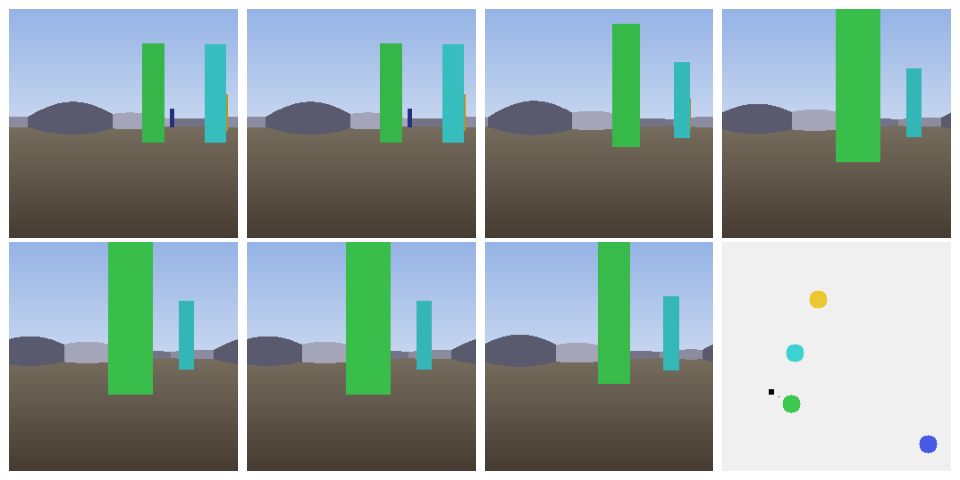
\includegraphics[width=0.49\linewidth]{fig/env_nav.png}\hfill
  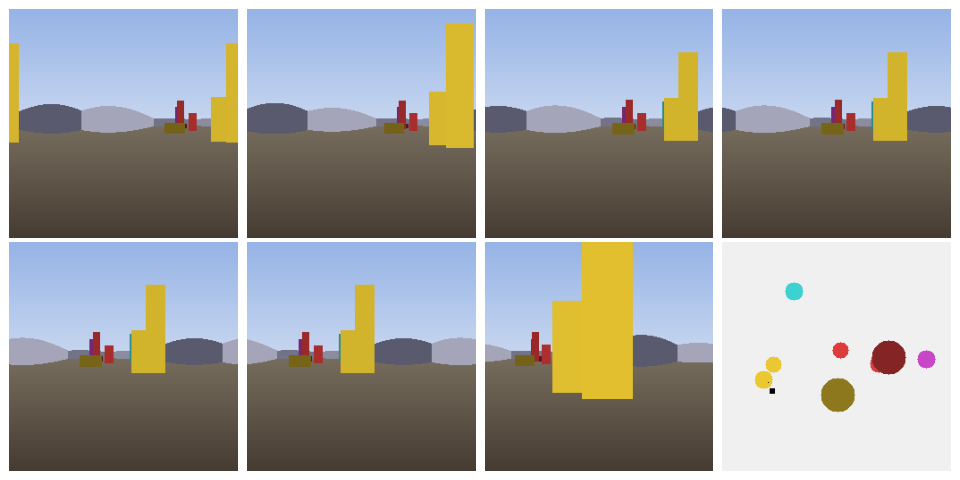
\includegraphics[width=0.49\linewidth]{fig/env_arrange.png}\\[2pt]
  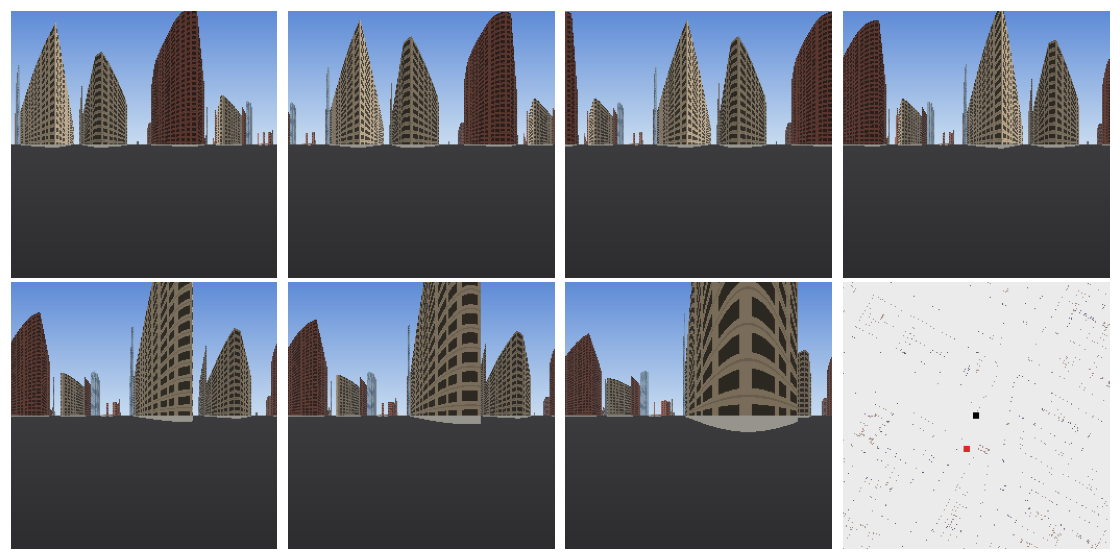
\includegraphics[width=\linewidth]{fig/env_nyc.png}\\[2pt]
  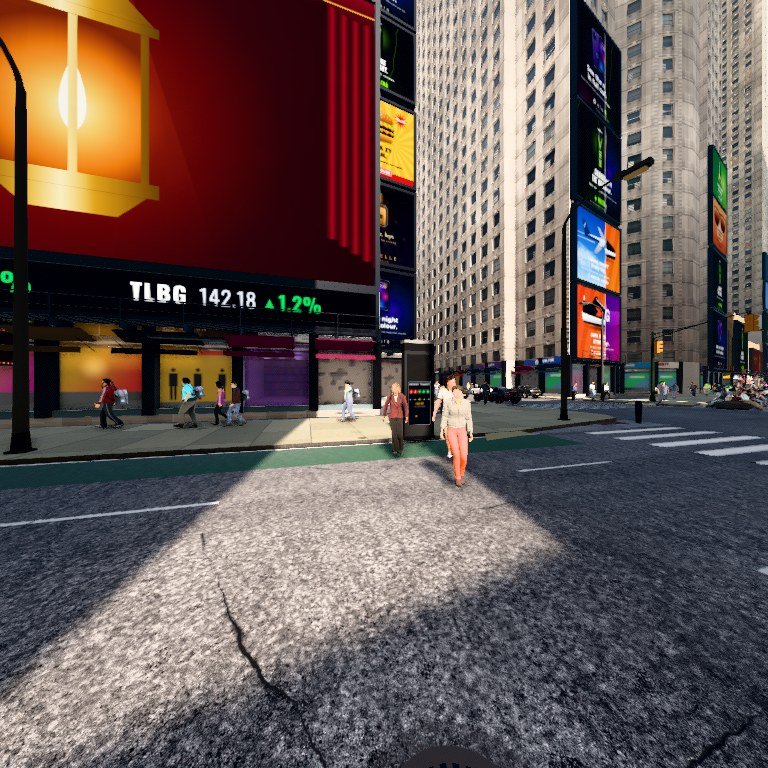
\includegraphics[width=\linewidth]{fig/nyc_hero_0.jpg}
  \caption{\textbf{Three worlds.} Top: the 360\degree\ arena for \textsc{nav} (left) and \textsc{arrange} (right).
  Bottom: seven steps of one episode in the raycast twin of Midtown Manhattan with its top-down map (start black,
  goal red), and the twin rendered at its highest quality (Times Square, ambient traffic and pedestrians). The third world, real phone video, is shown in \cref{fig:realvid}.}
  \label{fig:envs}
\end{figure}
\textbf{Arena.} A 360\degree\ cylindrical panorama at 256\,px with coloured blocks; tasks \textsc{nav} and
\textsc{arrange}; five actions (stay, forward 0.6, turn $\pm22.5$\degree, back 0.36); 24-step scripted episodes; 1,000
train, 200 test. \textbf{NYC twin.} A raycast model of Midtown Manhattan from building footprints; 110\degree\ camera,
forward 4\,m, back 2\,m, goals 30 to 60\,m; 600 episodes split \emph{geographically} into train and test street blocks.
\textbf{Real video.} \nRvClips\ phone clips walked through city streets, \nRvEpisodes\ episodes of 24 steps at 2\,Hz; yaw
and forward motion estimated by patch phase correlation and quantised to the five actions (\cref{sec:suppl-realvid}). A
test set only, except in the leave-one-clip-out fine-tuning condition. \textbf{Blackouts.} Test windows are steps 8 to
16 unless stated (also 8 to 24 and 4 to 24).

\paragraph{Metrics and probes}
Blind latent MSE and cosine in whitened PCA space, mean over horizons 1 to 8, against copy-last and constant-mean
floors. Ridge probes from $h_t$ to heading ($\sin,\cos$) and position relative to the start of the window, fit on
training episodes, reported as median heading error and position $R^2$, against two reference rows: \emph{actions
only} (the same probe on cumulative one-hot actions) and \emph{integrator} (closed-form dead reckoning, the
information ceiling). An MLP probe tests for non-linear codes. \emph{Blind homing}: 12 visible steps, then 24 steps
steered from a pose decoded from the state, success within 1 unit (12\,m on NYC), against oracle pose, dead reckoning
and random actions. \nSeeds\ seeds on the arena, \nSeedsNyc\ on NYC; mean\pm sd and 95\,\% $t$-intervals.

\section{Experiments}
\label{sec:exp}
Every number below is generated from the released result files by the table script in the repository; numbers that run 2 has not yet produced appear as red placeholders.

\subsection{Benchmark 1: blind latent prediction}
\label{sec:pred}
\begin{table*}[t]
  \centering\small
  \caption{\textbf{Blind latent prediction} (mean over horizons 1 to 8 in the 8:16 window; MSE in whitened PCA-256
  space, mean\pm sd over seeds). Lower MSE and higher cosine are better. Every student beats both trivial predictors.
  The GRU wins; the connectome beats every sparse control and the dense net on NYC but not the dense net on the arena.}
  \label{tab:pred}
  \resizebox{\linewidth}{!}{\begin{tabular}{lcccccc}
    \toprule
    & \multicolumn{2}{c}{Arena (5 seeds)} & \multicolumn{2}{c}{Cont.\ turns (0 seeds)} & \multicolumn{2}{c}{NYC twin (3 seeds)} \\
    \cmidrule(lr){2-3}\cmidrule(lr){4-5}\cmidrule(lr){6-7}
    wiring & MSE $\downarrow$ & cos $\uparrow$ & MSE $\downarrow$ & cos $\uparrow$ & MSE $\downarrow$ & cos $\uparrow$ \\
    \midrule
    GRU, parameter-matched & \textbf{0.434\pm0.004} & \textbf{0.72} & -- & -- & \textbf{0.609\pm0.003} & \textbf{0.56} \\
    GRU, recurrent-budget-matched & 0.501\pm0.001 & 0.67 & -- & -- & -- & -- \\
    dense & 0.562\pm0.004 & 0.63 & -- & -- & -- & -- \\
    connectome, unsigned & 0.573\pm0.001 & 0.63 & -- & -- & -- & -- \\
    connectome, random signs & 0.578\pm0.001 & 0.62 & -- & -- & -- & -- \\
    \textbf{connectome} & 0.579\pm0.003 & 0.62 & -- & -- & 0.701\pm0.010 & 0.47 \\
    random & 0.583\pm0.002 & 0.61 & -- & -- & 0.707\pm0.007 & 0.48 \\
    block-shuffled & 0.585\pm0.005 & 0.61 & -- & -- & 0.726\pm0.014 & 0.45 \\
    degree-shuffled & 0.610\pm0.002 & 0.59 & -- & -- & 0.731\pm0.005 & 0.45 \\
    \midrule
    copy last visible latent & 0.811 & -- & -- & -- & 1.558 & -- \\
    constant mean & 0.992 & -- & -- & -- & 0.977 & -- \\
    \bottomrule
\end{tabular}
}
\end{table*}
\Cref{tab:pred} is the result a world-model reader expects first and it does \emph{not} favour the wiring. The
parameter-matched GRU is \nGruBetterArena\,\% better than the connectome on the arena and \nGruBetterNyc\,\% on NYC;
even the GRU matched to the connectome's recurrent budget (174 units) is better. Among the sparse cores the ordering is
stable across seeds and worlds: connectome $<$ random $<$ block-shuffled $<$ degree-shuffled, with the real wiring
\nConnOverBlockArena\,\% ahead of block-shuffled on the arena and \nConnOverBlockNyc\,\% on NYC (paired over shared
test episodes, $p<0.001$ for every seed). Removing or permuting Dale's signs does not hurt prediction. Data efficiency
(50 to 1,000 training episodes) leaves the ordering unchanged (\cref{fig:curves}b, \cref{sec:suppl-data}).

\subsection{Benchmark 2: path integration read from the state}
\label{sec:probes}
\begin{figure*}[t]
  \centering
  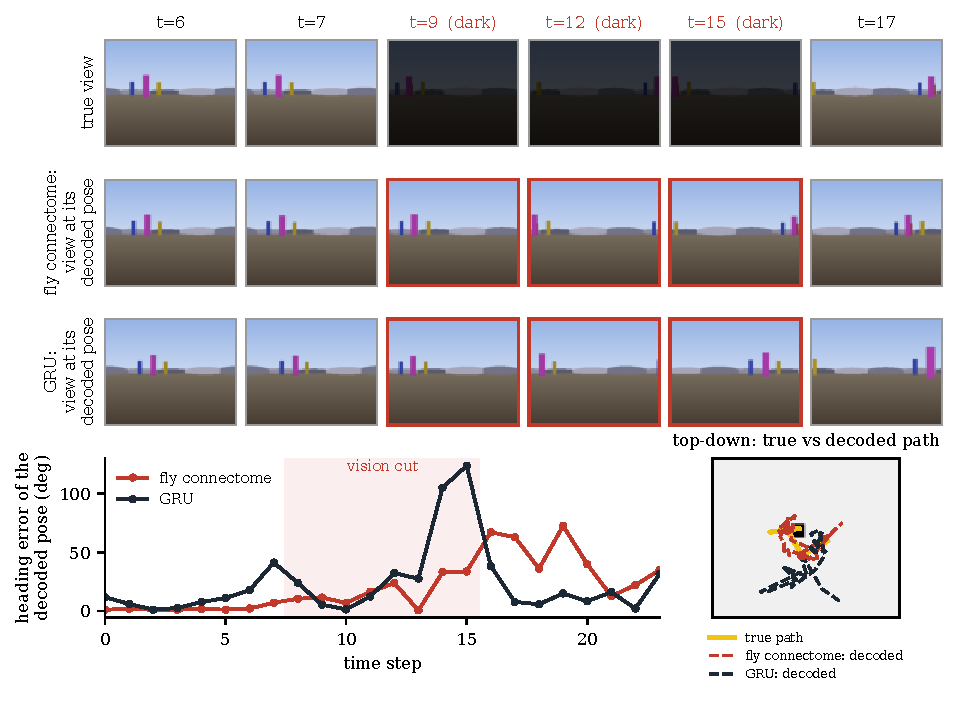
\includegraphics[width=\linewidth]{fig/video_strip.pdf}
  \caption{\textbf{What each network sees, thinks and decodes through a blackout} (one test episode closest to the
  population medians for both models). Top: the panorama the teacher receives, dimmed during the vision cut. Middle: the
  arena rendered at the pose a ridge readout decodes from each student's own activity, so each frame is where the network
  thinks it is. The connectome student's decoded view stays locked to the true view through the dark; the GRU's drifts.
  Bottom: heading error of the decoded pose over time, and the true path against both decoded paths. The readout never
  sees this episode.}
  \label{fig:strip}
\end{figure*}
\begin{table*}[t]
  \centering\small
  \caption{\textbf{Heading and position decoded from the state during 8 dark steps} (ridge probe; median heading
  error in degrees, position $R^2$; mean\pm sd over seeds). The integrator row is the information ceiling; the
  actions-only row is what a linear readout of the action history alone achieves.}
  \label{tab:probe}
  \resizebox{\linewidth}{!}{\begin{tabular}{lcccccc}
    \toprule
    & \multicolumn{2}{c}{Arena} & \multicolumn{2}{c}{Continuous turns} & \multicolumn{2}{c}{NYC twin} \\
    \cmidrule(lr){2-3}\cmidrule(lr){4-5}\cmidrule(lr){6-7}
    wiring & heading err & pos $R^2$ & heading err & pos $R^2$ & heading err & pos $R^2$ \\
    \midrule
    GRU, parameter-matched & 30.6\pm0.6 & 0.41\pm0.01 & -- & -- & 45.4\pm2.6 & 0.25\pm0.01 \\
    GRU, recurrent-budget-matched & 35.5\pm0.7 & 0.30\pm0.01 & -- & -- & -- & -- \\
    dense & 21.3\pm0.7 & 0.68\pm0.01 & -- & -- & -- & -- \\
    connectome, unsigned & 13.8\pm0.8 & 0.88\pm0.01 & -- & -- & -- & -- \\
    connectome, random signs & 9.2\pm1.3 & \textbf{0.94\pm0.01} & -- & -- & -- & -- \\
    \textbf{connectome} & \textbf{9.1\pm1.2} & 0.94\pm0.01 & -- & -- & \textbf{9.4\pm0.7} & \textbf{0.94\pm0.01} \\
    random & 12.9\pm0.7 & 0.88\pm0.01 & -- & -- & 15.1\pm0.7 & 0.89\pm0.00 \\
    block-shuffled & 10.8\pm0.8 & 0.93\pm0.01 & -- & -- & 10.1\pm1.1 & 0.94\pm0.02 \\
    degree-shuffled & 12.7\pm0.6 & 0.89\pm0.02 & -- & -- & 14.3\pm2.0 & 0.84\pm0.01 \\
    \midrule
    actions only (linear floor) & 40.1 & 0.54 & -- & -- & 22.6 & 0.41 \\
    integrator of the action record & 0.0 & 1.00 & -- & -- & 0.0 & 1.00 \\
    \bottomrule
\end{tabular}
}
\end{table*}
\begin{table*}[t]
  \centering\small
  \caption{\textbf{Longer dark windows and a non-linear probe} (arena; heading error, position $R^2$).}
  \label{tab:dark}
  \resizebox{\linewidth}{!}{\begin{tabular}{lcccc}
    \toprule
    wiring & ridge, 8 dark (8:16) & MLP, 8 dark & ridge, 16 dark (8:24) & ridge, 20 dark (4:24) \\
    \midrule
    GRU, parameter-matched & 30.6\pm0.6, 0.41 & 27.4\pm0.3, 0.42 & 37.7\pm0.8, 0.32 & 27.9\pm0.3, 0.50 \\
    GRU, recurrent-budget-matched & 35.5\pm0.7, 0.30 & 32.4\pm0.4, 0.32 & 44.8\pm0.5, 0.21 & 33.7\pm1.0, 0.35 \\
    dense & 21.3\pm0.7, 0.68 & 41.2\pm24.2, 0.27 & 29.9\pm1.1, 0.46 & 21.3\pm0.5, 0.53 \\
    connectome, unsigned & 13.8\pm0.8, 0.88 & -- & -- & -- \\
    connectome, random signs & 9.2\pm1.3, 0.94 & \textbf{4.7\pm0.3, 0.89} & 18.6\pm1.1, 0.82 & 13.6\pm1.4, 0.82 \\
    \textbf{connectome} & \textbf{9.1\pm1.2, 0.94} & 4.7\pm0.1, 0.87 & \textbf{17.7\pm2.1, 0.82} & \textbf{12.6\pm1.2, 0.82} \\
    random & 12.9\pm0.7, 0.88 & 6.4\pm0.4, 0.83 & 24.9\pm0.6, 0.72 & 17.3\pm0.6, 0.77 \\
    block-shuffled & 10.8\pm0.8, 0.93 & 5.9\pm0.3, 0.86 & 23.3\pm0.4, 0.77 & 15.9\pm0.6, 0.77 \\
    degree-shuffled & 12.7\pm0.6, 0.89 & 6.9\pm0.7, 0.83 & 24.0\pm1.0, 0.71 & 17.2\pm0.6, 0.76 \\
    \bottomrule
\end{tabular}
}
\end{table*}
\Cref{tab:probe} is where the wiring pays. The connectome state yields \nConnArenaHd\degree\ median heading error and
position $R^2$ \nConnArenaPos\ on the arena and \nConnNycHd\degree\ / \nConnNycPos\ on NYC; the GRU, which predicts the
latent far better, gives \nGruArenaHd\degree\ / \nGruArenaPos\ and \nGruNycHd\degree\ / \nGruNycPos. Four controls
make the reading safe. (i) The actions-only floor is \nActOnlyArenaHd\degree, so the probe is reading an integral held
by the state, not the raw action input. (ii) A random 762-neuron subset of the connectome (the GRU's width) still beats
the GRU, so feature count is not the explanation (\cref{sec:suppl-probe}). (iii) An MLP probe tightens the connectome
to \nConnArenaMlpHd\degree\ and the GRU only to \nGruArenaMlpHd\degree\ (\cref{tab:dark}), so the GRU's code is not
merely non-linear. (iv) With continuous turn angles the action record no longer determines heading; the continuous-turn probe columns of
\cref{tab:probe} are filled by run 2 (\nSeedsTn\ seeds at the time of writing), and the homing result on that data is
already in \cref{tab:homing}. The code degrades gracefully (\cref{fig:curves}a, \cref{fig:strip}): at 16 dark steps the connectome holds
\nConnArenaDarkSixteenHd\degree\ against \nGruArenaDarkSixteenHd\degree\ for the GRU, and the real wiring's margin over
block-shuffled grows from \nConnBlockGapArena\degree\ to \nConnBlockGapArenaDarkSixteen\degree. Signs matter here where
they did not for prediction: the unsigned graph loses 5\degree. The 51 EPG neurons alone carry almost no heading
($R^2<0.2$); no ring attractor emerges at this scale.

\subsection{Single versus multiple connectomes}
\label{sec:multi}
\begin{figure*}[t]
  \centering
  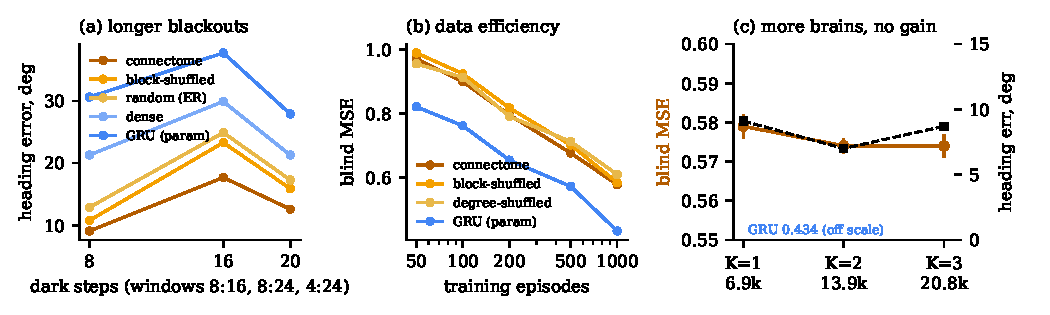
\includegraphics[width=\linewidth]{fig/curves.pdf}
  \caption{\textbf{Robustness of the two findings.} (a) The dark heading code degrades gracefully with the blackout
  length and the sparse-versus-free ordering never changes. (b) From 50 to 1,000 training episodes the GRU leads and the
  connectome beats block-shuffled at every size; a prior that should matter most with little data does not change the
  ranking. (c) Coupling two or three copies of the brain through the real commissural synapses adds neurons but no
  accuracy and leaves the heading code where it was.}
  \label{fig:curves}
\end{figure*}
\begin{table}[t]
  \centering\small
  \caption{\textbf{Multi-brain scaling} (arena, 5 seeds). $K$ copies coupled through the real commissural synapses.}
  \label{tab:multi}
  \begin{tabular}{lcccc}
    \toprule
    $K$ & neurons & synapses & blind MSE & heading err \\
    \midrule
    1 & 6,935 & 91,663 & 0.579\pm0.003 & 9.1\pm1.2 \\
    2 & 13,870 & 183,326 & 0.574\pm0.002 & 7.0 \\
    3 & 20,805 & 274,989 & 0.574\pm0.003 & 8.7 \\
    \bottomrule
  \end{tabular}
\end{table}
Doubling or tripling the brain (\cref{tab:multi}, \cref{fig:curves}c) changes blind MSE by less than one seed standard deviation and
leaves the heading code where it was. The sparse student is therefore not short of neurons or synapses; the gap to
the GRU is a property of the fixed sparse topology, not of its size. One real brain is enough, and we use $K=1$
everywhere else.

\subsection{Sparse state versus dense state: where the gap lives}
\label{sec:gap}
Two thirds of the sparse student's parameters are in the shared linear input map. Replacing it by the cross-attention
encoder, which removes 1.7\,M parameters from every architecture, leaves both the prediction gap and the
path-integration gap in place (\nConnAttnArenaMse\ / \nConnAttnArenaHd\degree\ for the connectome,
\nGruAttnArenaMse\ / \nGruAttnArenaHd\degree\ for the GRU). Adding one attention layer over cell-type tokens to the
connectome recurrence brings MSE to \nHybridArenaMse\ and heading to \nHybridArenaHd\degree. The dense recurrence on
the same neurons predicts better than the connectome (0.562 vs 0.579) but integrates far worse (21\degree\ vs
9\degree), which places it between the two families, exactly where its free weights put it.

\subsection{Benchmark 3: behaviour from the code}
\label{sec:behaviour}
\begin{figure*}[t]
  \centering
  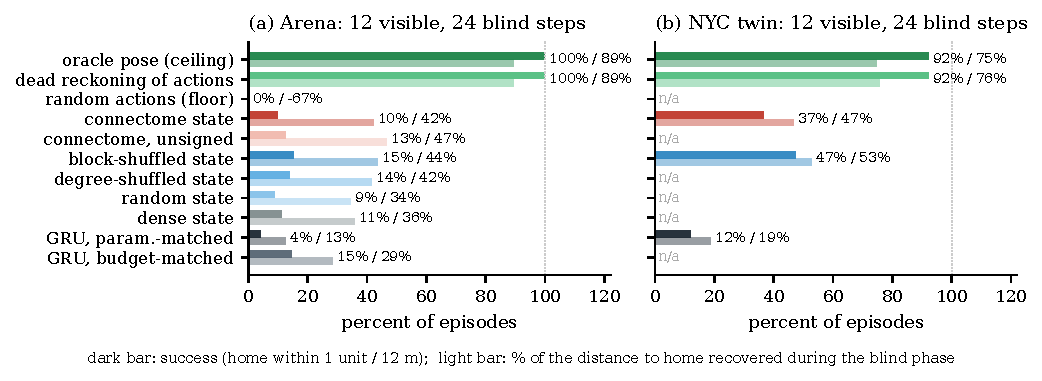
\includegraphics[width=\linewidth]{fig/homing.pdf}
  \caption{\textbf{Blind homing.} After 12 visible steps vision is cut and the same controller steers for 24 steps from
  one of several pose estimates. With the true pose or dead reckoning it gets home almost every time, so the controller
  is not the limit. From a linear readout of a connectome-sized sparse state the agent recovers about half the distance;
  from the GRU state it barely moves. The real wiring has no edge over block-shuffled here.}
  \label{fig:homing}
\end{figure*}
\begin{table*}[t]
  \centering\small
  \caption{\textbf{Blind homing} from a pose decoded linearly from the state (\% of start distance recovered; success
  within 1 unit / 12\,m).}
  \label{tab:homing}
  \resizebox{\linewidth}{!}{\begin{tabular}{lcccccc}
    \toprule
    & \multicolumn{2}{c}{Arena} & \multicolumn{2}{c}{Continuous turns} & \multicolumn{2}{c}{NYC twin} \\
    \cmidrule(lr){2-3}\cmidrule(lr){4-5}\cmidrule(lr){6-7}
    pose readout & \% closer & success & \% closer & success & \% closer & success \\
    \midrule
    oracle pose (controller ceiling) & 89 & 1.00 & -- & -- & 75 & 0.92 \\
    dead reckoning of actions & 89 & 1.00 & 87 & 0.90 & 76 & 0.92 \\
    random actions (floor) & -67 & 0.00 & -- & -- & -- & -- \\
    \midrule
    GRU, parameter-matched state & 13 & 0.04 & 21 & 0.16 & 19 & 0.12 \\
    GRU, recurrent-budget-matched state & 29 & 0.15 & -- & -- & -- & -- \\
    dense state & 36 & 0.11 & -- & -- & -- & -- \\
    connectome, unsigned state & \textbf{47} & 0.13 & -- & -- & -- & -- \\
    \textbf{connectome} state & 42 & 0.10 & \textbf{33} & \textbf{0.16} & 47 & 0.37 \\
    random state & 34 & 0.09 & -- & -- & -- & -- \\
    block-shuffled state & 44 & \textbf{0.15} & -- & -- & \textbf{53} & \textbf{0.47} \\
    degree-shuffled state & 42 & 0.14 & -- & -- & -- & -- \\
    \bottomrule
\end{tabular}
}
\end{table*}
A linear readout of the connectome state drives blind homing to \nConnNycSucc\ success on NYC and \nConnArenaSucc\ on
the arena (\cref{tab:homing}, \cref{fig:homing}), well above the random-action floor and the GRU (\nGruNycSucc, \nGruArenaSucc) but far
below the dead-reckoning ceiling (0.92, 1.00). Block-shuffled homes slightly better than the real wiring. Goal-vector
navigation toward a decoded goal does not beat random actions. The controller is not the bottleneck (the oracle pose
reaches the ceiling); the readout is.

\subsection{Benchmark 4: real handheld video}
\label{sec:realvid}
\begin{figure*}[t]
  \centering
  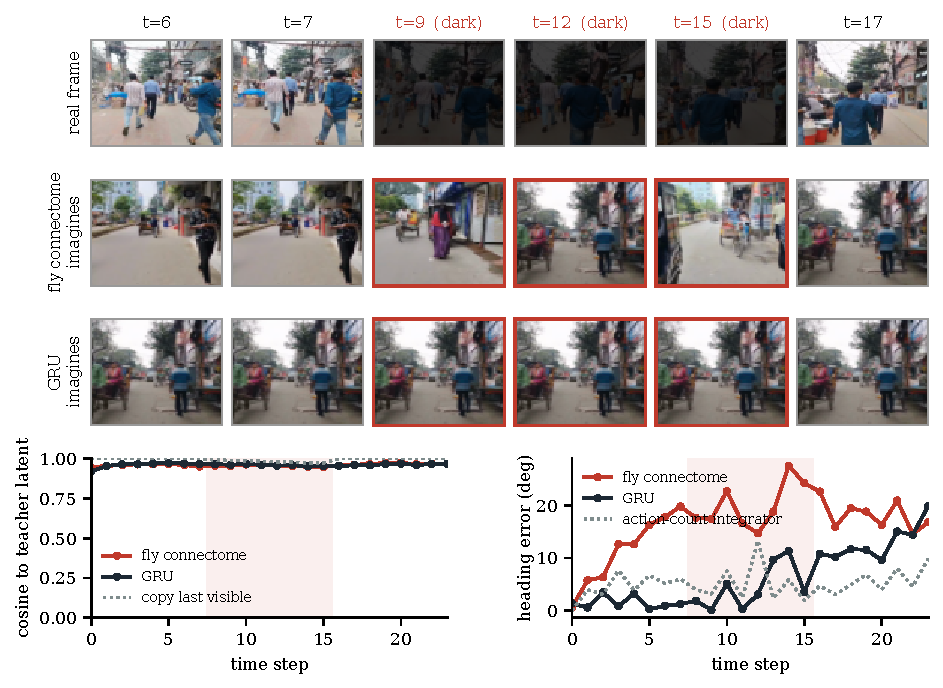
\includegraphics[width=\linewidth]{fig/realvid_strip.pdf}
  \caption{\textbf{The same test on real handheld video} (one held-out phone clip; both students fine-tuned on the other
  clips). Top: the real frame, dimmed during the vision cut. Middle: the training frame whose teacher latent is nearest
  to each student's guess, \ie what each imagines. Bottom left: cosine to the teacher latent against a copy-last
  baseline (dotted). Bottom right: heading decoded from the state against the clip's own egomotion estimate.}
  \label{fig:realvid}
\end{figure*}
\begin{figure}[t]
  \centering
  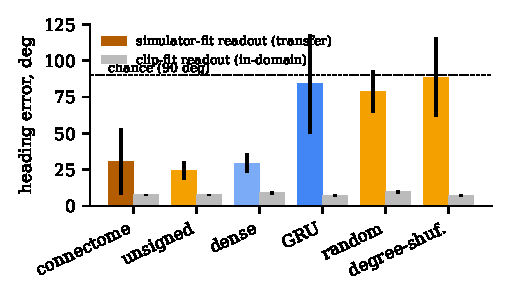
\includegraphics[width=\linewidth]{fig/realvid_bars.pdf}
  \caption{\textbf{Does the heading code transfer from simulator to phone video?} Heading error on real clips with a
  readout fit in the simulator (coloured) or on the other clips (grey). The connectome, unsigned and dense states
  transfer; the GRU, random and degree-shuffled states fall to chance.}
  \label{fig:rvbars}
\end{figure}
\begin{table*}[t]
  \centering\small
  \caption{\textbf{Real phone video} (\nRvClips\ clips, \nRvEpisodes\ episodes): zero-shot and leave-one-clip-out
  fine-tuned MSE, and heading probes with the simulator-fit readout (transfer) or a readout fit on the other clips.}
  \label{tab:realvid}
  \resizebox{\linewidth}{!}{\begin{tabular}{lcccccc}
    \toprule
    wiring & zero-shot MSE & fine-tuned MSE & heading, sim.\ readout & heading, clip readout & NYC model, zero-shot & NYC model, fine-tuned \\
    \midrule
    GRU, parameter-matched & 9.94\pm0.07 & \textbf{1.18\pm0.00} & 84.1\pm34.2 & 7.6\pm0.7 & \textbf{5.57\pm0.03} & -- \\
    dense & 9.73\pm0.07 & 1.21\pm0.04 & 29.5\pm6.4 & 9.1\pm0.9 & -- & -- \\
    connectome, unsigned & 9.59\pm0.13 & 1.26\pm0.00 & \textbf{24.3\pm6.3} & 7.7\pm0.3 & -- & -- \\
    \textbf{connectome} & 9.68\pm0.10 & 1.24\pm0.02 & 30.9\pm22.8 & 7.7\pm0.5 & 6.10\pm0.03 & -- \\
    random & \textbf{9.56\pm0.19} & 1.26\pm0.01 & 79.1\pm14.5 & 9.9\pm1.1 & 6.00\pm0.02 & -- \\
    degree-shuffled & 9.69\pm0.09 & 1.25\pm0.02 & 88.7\pm27.0 & \textbf{7.1\pm0.6} & 6.01\pm0.05 & -- \\
    \midrule
    copy last visible latent & 0.84 & 0.84 & -- & -- & 0.84 & 0.84 \\
    constant mean & 10.28 & 10.28 & -- & -- & 10.28 & 10.28 \\
    actions only (linear floor) & -- & -- & -- & 4.7 & -- & -- \\
    \bottomrule
\end{tabular}
}
\end{table*}
Zero-shot, no student beats the copy-last predictor on real footage (\cref{tab:realvid}): the simulator-to-phone gap
swamps every architectural difference. After fine-tuning all students land within 7\,\% of each other. The heading
probe is the informative row (\cref{fig:rvbars}): with the \emph{simulator-fit} readout the connectome and unsigned connectome transfer at
\nConnArenaRvTransferHd\degree\ and \nNosignArenaRvTransferHd\degree\ while the GRU, random and degree-shuffled states
do not transfer at all (79 to 89\degree); with an in-domain readout every state decodes heading to 7 to 10\degree.

\subsection{What is outperformed, and what is not}
\label{sec:scorecard}
\begin{table}[t]
  \centering\footnotesize
  \caption{\textbf{Scorecard.} Does the connectome beat each baseline on each benchmark? \checkmark\ yes (5 seeds,
  paired $p<0.01$); $\approx$ within seed noise; $\times$ no.}
  \label{tab:score}
  \setlength{\tabcolsep}{3pt}\begin{tabular}{lcccc}
    \toprule
    baseline & MSE & heading & homing & real-video \\
    \midrule
    degree-shuffled & \checkmark & \checkmark & $\approx$ & \checkmark \\
    random (ER) & \checkmark & \checkmark & \checkmark & \checkmark \\
    block-shuffled & \checkmark & \checkmark & $\times$ & -- \\
    random signs & $\approx$ & $\approx$ & -- & -- \\
    unsigned & $\times$ & \checkmark & $\times$ & $\approx$ \\
    dense & $\times$ & \checkmark & \checkmark & $\approx$ \\
    GRU (param-matched) & $\times$ & \checkmark & \checkmark & \checkmark \\
    GRU (recurrent-matched) & $\times$ & \checkmark & \checkmark & -- \\
    transformer & $\times$ & \checkmark & -- & -- \\
    \bottomrule
  \end{tabular}
\end{table}
\Cref{tab:score} condenses the paper. The connectome beats every \emph{wiring} control on prediction and on the dark
heading code. It loses prediction to every \emph{free} recurrence and wins the dark heading code against all of them.

\subsection{Cost, scaling and ablation}
\label{sec:more}
One connectome step costs 7.4\,MFLOP, the same as the parameter-matched GRU, with 91,663 recurrent weights against
the GRU's 580,644; dense costs 103\,MFLOP. With the synapse threshold at 1, 5 or 10, with MB or OUT removed, or with CX
alone, the real wiring beats its degree-shuffled twin by 0.02 to 0.04 MSE (\cref{sec:ablation}); no single region
carries the margin.

\section{Where the novelty lies}
\label{sec:novelty}
Stated as claims a reviewer can check against the tables:
\begin{enumerate}
  \item \textbf{A new student class for world-model distillation.} Prior distillation changes the size or the family
        of the student but leaves its recurrence free. Here the recurrence is a fixed, signed, synapse-level wiring
        diagram from a real animal, and the distillation target is a self-supervised video foundation model rather
        than a task loss or neural recordings (\cref{tab:prior}).
  \item \textbf{A control ladder that separates four things usually conflated:} density (dense vs sparse), degree
        sequence (degree-shuffled), macro-architecture (block-shuffled) and synapse identity (real). The result is
        quantitative: identity is worth about 1\,\% of latent error and 2 to 6\degree\ of heading, reproducibly
        (\cref{tab:pred,tab:dark}).
  \item \textbf{An emergent path-integration code that prediction quality does not explain.} The best predictors keep
        the least heading. The code forms in connectome-scale sparse signed recurrence trained only on latent
        prediction, survives 20 dark steps, continuous turns, a non-linear probe and a geographic train/test split, and
        transfers from simulator to phone video where the GRU's does not (\cref{tab:probe,tab:dark,tab:realvid}).
  \item \textbf{A single-vs-multi-connectome result.} Cloning the brain through its 40,194 real commissural synapses
        is a new, control-preserving way to scale a connectome model, and it shows the student is topology-limited
        rather than size-limited (\cref{tab:multi}).
  \item \textbf{Three worlds and a full negative-result record.} Arena, a geographically split city twin and real
        footage; blind homing and goal-vector navigation with ceilings and floors; nothing is left out because it
        failed.
\end{enumerate}

\section{Discussion}
\label{sec:discussion}
\paragraph{Two claims that are easy to conflate}
The first is about a \emph{class} of topology: connectome-scale sparse signed recurrence, trained only to predict a
video model's latent, holds a state that path-integrates, and neither a GRU nor a transformer trained on the same
objective at the same budget does, even under a non-linear probe and an equalised input encoder. We find this strong
because both predict the latent better; the code trades against prediction rather than following from it. The second
is about the \emph{identity} of the real synapses, and here the evidence is modest and consistent: about one percent of
latent error, a few degrees of heading, present across seeds, worlds, data sizes and subgraphs, but never the cause and
absent from the behavioural readouts. A reader who takes away ``sparse signed recurrence integrates, and the fly's
version is a little better'' has understood the paper.

\paragraph{Why might sparse recurrence integrate}
A hypothesis, not a proof. A large sparse signed graph has a reservoir of slow, weakly coupled modes. The leaky update
drives those modes with the action input, and the linear readout can leave them alone because they cost almost
nothing in latent error. A gated unit with a dense $762^2$ recurrence, or a transformer that can re-read its visible
past, is pushed by the same objective to spend capacity on prediction, and nothing in the loss rewards keeping an
integral around. The probes on random and shuffled sparse graphs fit this picture.

\paragraph{Proposed direction}
\begin{itemize}
  \item \textbf{Mechanism.} Spectral analysis of the trained $W$, lesions of its slow modes, and a per-cell-type
        decomposition of the heading code, to turn the hypothesis above into a test.
  \item \textbf{Close the readout gap.} Homing sits at 37\,\% against a 92\,\% ceiling with a linear readout. A
        recurrent or learned controller fit on more closed-loop rollouts is the obvious next step; the oracle result
        shows the search is not the problem.
  \item \textbf{Egomotion from vision.} Both simulators hand the student its actions in the dark. Estimating
        self-motion from optic flow inside the VIS population would remove the last trivial information path.
  \item \textbf{Scale the teacher and the footage.} ViT-L at 384\,px, and 30 minutes of walking video with real
        odometry (RECON- or SCAND-style) so the flow-estimated actions can be validated.
  \item \textbf{Hybrid cores.} The one-layer attention hybrid asks whether global routing is what the sparse graph
        lacks; a graded family between connectome and transformer would map the trade-off curve in \cref{fig:main}.
\end{itemize}

\paragraph{Limitations}
(i) Behavioural readouts are linear, and that is where the result stops short. (ii) On the fixed-turn arena the
information ceiling is trivial; continuous turns remove it, but actions are still given. (iii) The environments are
synthetic, and on real video no student beats copy-last zero-shot. (iv) The teacher is ViT-B at 256\,px. (v) The NYC
twin uses one location. (vi) The EPG population does not carry the heading code; the biological ring attractor does
not emerge at this scale and we do not claim it.

\paragraph{Broader impact}
The connectome is released by \flywire under CC-BY-NC~4.0; our derived graph inherits that licence and is rebuilt by
one script rather than redistributed. No human data are used. The methodological lesson is that biological wiring is a
source of structural priors to be tested with matched controls, not a blueprint to be copied, and the controls are
where most of the information is.

\section{Conclusion}
A video foundation model can be distilled into a world model whose recurrence is the fly's wiring diagram. The wiring
makes it a worse predictor and a better integrator: the state keeps a linearly readable heading and position through
the dark that neither a GRU nor a transformer trained on the same objective forms, with a small, consistent advantage
for the real synapses over shuffled ones, and no gain from adding more brains. Turning that code into reliable blind
behaviour is the open problem, and we release everything needed to work on it.

{\small
\bibliographystyle{ieeenat_fullname}
\bibliography{main}}
\clearpage
\appendix
\section{Supplementary material}

\subsection{Extended probe results}
\label{sec:suppl-probe}
\cref{tab:suppl-probe} gives the per-population and feature-count-matched probes for the arena (seed 0), the MLP
probe on all wirings, and the NYC dark-duration numbers. ``all@762'' is a random 762-neuron subset of the student,
the GRU's width; ``rand@CX'' is a random subset the size of the central complex.

\begin{table}[h]
  \centering\small
  \setlength{\tabcolsep}{3pt}
  \resizebox{\linewidth}{!}{%
\begin{tabular}{lcccccc}
    \toprule
    wiring & all & all@762 & CX & rand@CX & EPG & MLP, all \\
    \midrule
    connectome & 8.5 & 18.9 & 12.6 & 10.7 & 50.1 & 4.7\pm0.1 \\
    connectome, random signs & 7.9 & 16.8 & 11.7 & 10.4 & 44.0 & 4.7\pm0.3 \\
    block-shuffled & 11.1 & 20.9 & 14.4 & 13.2 & 38.5 & 5.9\pm0.3 \\
    degree-shuffled & 12.6 & 20.1 & 14.1 & 15.0 & 35.2 & 6.9\pm0.7 \\
    random & 12.8 & 19.2 & 14.5 & 14.4 & 37.3 & 6.4\pm0.4 \\
    connectome, unsigned & 12.8 & 20.6 & 13.9 & -- & 34.2 & -- \\
    dense & 21.5 & 28.8 & 25.2 & 23.7 & 39.8 & 41\pm24 \\
    GRU, parameter-matched & 31.6 & -- & -- & -- & -- & 27.4\pm0.3 \\
    GRU, recurrent-budget-matched & 35.2 & -- & -- & -- & -- & -- \\
    \bottomrule
  \end{tabular}}
  \caption{Median heading error (\degree) in the 8:16 blind window, arena, seed 0 (MLP column: mean\pm sd over 3
  seeds). The EPG population alone carries almost no heading; the central complex decodes no better than a random
  subset of its size.}
  \label{tab:suppl-probe}
\end{table}

\begin{table}[h]
  \centering\small
  \resizebox{\linewidth}{!}{%
\begin{tabular}{lcc}
    \toprule
    wiring (NYC) & 16 dark (8:24) & 20 dark (4:24) \\
    \midrule
    connectome & 12.2\pm2.2, 0.88 & 9.5\pm1.3, 0.88 \\
    block-shuffled & 16.4\pm1.5, 0.86 & 12.2\pm2.0, 0.84 \\
    degree-shuffled & 25.2\pm1.8, 0.69 & 15.9\pm0.7, 0.73 \\
    random & 21.6\pm1.1, 0.80 & 14.0\pm0.3, 0.83 \\
    GRU, parameter-matched & 49.4\pm1.9, 0.08 & 39.8\pm1.5, 0.25 \\
    \bottomrule
  \end{tabular}}
  \caption{Dark duration on the NYC twin: heading error (\degree) and position $R^2$, ridge probe, 3 seeds.}
  \label{tab:suppl-dark-nyc}
\end{table}

\subsection{Goal-vector navigation}
\label{sec:suppl-goalnav}
\begin{table}[h]
  \centering\small
  \setlength{\tabcolsep}{3pt}
  \resizebox{\linewidth}{!}{%
\begin{tabular}{llcccc}
    \toprule
    wiring & env & readout & no cut & cut 3 & cut 5 \\
    \midrule
    connectome & arena & oracle goal vector & 0.92 / 0.70 & 0.92 / 0.70 & 0.92 / 0.70 \\
    connectome & arena & random actions & 0.14 / 0.12 & 0.14 / 0.12 & 0.14 / 0.12 \\
    connectome & arena & state (ridge) & 0.22 / 0.16 & 0.22 / 0.15 & 0.22 / 0.14 \\
    connectome & arena & state (MLP) & 0.24 / 0.15 & -- & -- \\
    block-shuffled & arena & state & 0.24 / 0.15 & 0.23 / 0.14 & 0.21 / 0.13 \\
    degree-shuffled & arena & state & 0.22 / 0.13 & 0.23 / 0.14 & 0.21 / 0.13 \\
    random & arena & state & 0.21 / 0.13 & 0.21 / 0.12 & 0.19 / 0.12 \\
    dense & arena & state & 0.20 / 0.12 & 0.21 / 0.12 & 0.22 / 0.12 \\
    GRU, param.-matched & arena & state & 0.22 / 0.15 & 0.22 / 0.14 & 0.22 / 0.16 \\
    GRU, budget-matched & arena & state & 0.23 / 0.14 & 0.23 / 0.11 & 0.23 / 0.13 \\
    \midrule
    connectome & NYC, greedy & oracle & 0.28 / 0.25 & -- & 0.28 / 0.25 \\
    connectome & NYC, greedy & state & 0.05 / 0.05 & -- & 0.04 / 0.04 \\
    \midrule
    connectome & NYC, bumper & oracle & 0.83 / 0.78 & 0.83 / 0.78 & 0.83 / 0.78 \\
    connectome & NYC, bumper & random actions & 0.00 / 0.00 & 0.00 / 0.00 & 0.00 / 0.00 \\
    connectome & NYC, bumper & state (ridge) & 0.18 / 0.18 & 0.21 / 0.21 & 0.17 / 0.17 \\
    connectome & NYC, bumper & state (MLP) & 0.27 / 0.25 & -- & -- \\
    block-shuffled & NYC, bumper & state & 0.10 / 0.10 & 0.14 / 0.14 & 0.13 / 0.13 \\
    random & NYC, bumper & state & 0.06 / 0.05 & 0.02 / 0.02 & 0.04 / 0.04 \\
    transformer & NYC, bumper & state & 0.16 / 0.15 & 0.14 / 0.14 & 0.16 / 0.15 \\
    GRU, param.-matched & NYC, bumper & state & 0.11 / 0.11 & 0.11 / 0.11 & 0.12 / 0.12 \\
    GRU, param.-matched & NYC, bumper & state (MLP) & 0.17 / 0.16 & -- & -- \\
    \midrule
    connectome & NYC dusk / overcast / fog / night & state & 0.23 / 0.20 / 0.17 / 0.13 & -- & -- \\
    block-shuffled & NYC dusk / overcast / fog / night & state & 0.13 / 0.10 / 0.10 / 0.00 & -- & -- \\
    transformer & NYC dusk / overcast / fog / night & state & 0.13 / 0.17 / 0.13 / 0.17 & -- & -- \\
    GRU, param.-matched & NYC dusk / overcast / fog / night & state & 0.13 / 0.13 / 0.20 / 0.13 & -- & -- \\
    \bottomrule
  \end{tabular}}
  \caption{Goal-vector navigation: success / SPL~\cite{anderson2018evaluation}. Arena: 50 episodes per seed, 3 seeds.
  NYC: 30 episodes per seed, 3 seeds for state readouts, goals 30 to 60\,m. The vision cut lasts 3 or 5 steps from
  step 6. With the greedy controller even the oracle goal vector fails on streets (it walks into buildings), so the NYC
  rows use a bumper controller (on collision: turn two steps toward the goal side, commit three steps forward), which
  lifts the oracle to 0.83. Under it the state readouts clear random actions and random wiring, the connectome is the
  best core (0.18 ridge, 0.27 MLP, seed 0), and the vision cut barely matters: the readout, not vision loss, is the
  limit. The last block is the clear-trained readout evaluated under appearance shifts (seed 0, success only).}
  \label{tab:goalnav}
\end{table}

\subsection{Data efficiency}
\label{sec:suppl-data}
\begin{table}[h]
  \centering\small
  \resizebox{\linewidth}{!}{%
\begin{tabular}{lcccc}
    \toprule
    train episodes & connectome & block-shuffled & degree-shuffled & GRU \\
    \midrule
    50 & 0.970\pm0.009 & 0.989\pm0.009 & 0.955\pm0.013 & \textbf{0.821\pm0.007} \\
    100 & 0.899\pm0.003 & 0.924\pm0.006 & 0.913\pm0.003 & \textbf{0.762\pm0.016} \\
    200 & 0.796\pm0.011 & 0.818\pm0.021 & 0.791\pm0.009 & \textbf{0.655\pm0.007} \\
    500 & 0.677\pm0.003 & 0.702\pm0.015 & 0.713\pm0.004 & \textbf{0.573\pm0.002} \\
    1000 & 0.579\pm0.003 & 0.585\pm0.005 & 0.610\pm0.002 & \textbf{0.434\pm0.004} \\
    \bottomrule
  \end{tabular}}
  \caption{Blind MSE (arena, mean over horizons, 3 seeds; 5 at 1000) against training-set size. PCA basis fit on the
  full training set in every row.}
  \label{tab:data}
\end{table}

\subsection{Subgraph ablation}
\begin{table}[h]
  \centering\small
  \resizebox{\linewidth}{!}{%
\begin{tabular}{lccc}
    \toprule
    subgraph & connectome & degree-shuffled & margin \\
    \midrule
    full graph ($\ge$5 synapses, 91,663 edges) & 0.575 & 0.610 & 0.035 \\
    $\ge$1 synapse & 0.618 & 0.661 & 0.043 \\
    $\ge$10 synapses & 0.584 & 0.604 & 0.020 \\
    central complex only & 0.588 & 0.608 & 0.020 \\
    mushroom bodies removed & 0.582 & 0.609 & 0.027 \\
    descending neurons removed & 0.588 & 0.610 & 0.022 \\
    \bottomrule
  \end{tabular}}
  \caption{Blind MSE 8:16, arena, seed 0, real wiring against the degree-shuffled rewiring of the same subgraph. The
  full-graph margin is 0.035\pm0.005 over 5 seeds.}
  \label{tab:ablation}\label{sec:ablation}
\end{table}

\subsection{Real handheld video}
\label{sec:suppl-realvid}
The clips are walked with a phone held at chest height; each is centre-cropped to a square, resampled to 2\,Hz and cut
into non-overlapping 24-step episodes. Yaw per step is the mean horizontal phase-correlation shift over a $4\times4$
patch grid converted through a 60\degree\ horizontal field of view; forward motion is the mean radial expansion. Steps
with $|{\rm yaw}| > 6^\circ$ become turn actions, steps with expansion above 1\,px forward, below $-1$\,px back, the
rest stay. The heading target of the probe is the integrated continuous yaw, not the quantised record, so the
``actions only'' floor and the probe measure different things on this data. Zero-shot, fine-tuned and probe numbers for
every architecture are in \cref{tab:realvid}; per-clip numbers are in \texttt{results/summary.md}.

\subsection{Teacher-free planning (negative)}
\label{sec:suppl-plan}
Latent CEM-MPC with the student as dynamics model succeeds in 0 to 3\,\% of arena navigation episodes for every
wiring, while the same planner with oracle dynamics succeeds in 100\,\% and a scripted policy in 100\,\%; on the NYC
twin student-model planning is at 0\,\% under clear, dusk, night, fog and overcast appearance. The students' 8-step
rollouts are not accurate enough to plan with. Dropped from the claims.

\subsection{Video}
The supplementary video (\texttt{wm2cx\_paper.mp4}, generated by \texttt{scripts/make\_video\_paper.py}) shows one
arena episode side by side for the \vjepa teacher, the connectome-wired student and the parameter-matched GRU: what each
receives (panorama, fly-eye input, neuron or hidden-unit activity), what each thinks (its latent guess on the teacher's
2-D latent trajectory, with the cosine match over time) and where each believes it is (the pose decoded from its own
state, the view rendered there, and the decoded path on the top-down map). The released strip figures are cut from it. A second
video (\texttt{wm2cx\_realvid.mp4}, \texttt{scripts/make\_video\_realvid.py}) repeats the comparison on a held-out real
phone clip with both students fine-tuned on the other clips.

\subsection{Reproducibility}
All results in the paper come from one run on a single RTX 4090 (about 14 GPU-hours): 5 seeds on the arena, 3 on NYC,
12 wirings, 424 checkpoints. Code, environments, the ingest pipeline for phone video, and the checkpoints are released;
the \flywire-derived connectome file is rebuilt by one script from the public v783 release.

\end{document}
